% =====================================================================
% 1. ADVANCED SYSTEM PREAMBLE (COMPILATION TOPOLOGY LAYOUT)
% =====================================================================
\documentclass[11pt,twoside,letterpaper]{article}

% --- Core System Engine Packages ---
\usepackage{fontspec}           % Advanced system font manager (XeLaTeX/LuaLaTeX required)
\usepackage{geometry}           % Page margin grid configuration layouts
\geometry{letterpaper, margin=1in, bindingoffset=0in}
\usepackage{amsmath, amssymb}   % Structural math fonts and set-theory delimiters
\usepackage{listings}           % Advanced code block container for Sanskrit/Python scripts
\usepackage{microtype}          % Fine-tuned typographic spacing adjustments
\usepackage{graphicx}           % Core graphics engine for images and diagrams
\usepackage[dvipsnames,table]{xcolor} % Loads extended color names (teal, slate, blue)

% --- Unified Citation and Link Routing Configurations (Natbib Engine) ---
\usepackage[round,authoryear]{natbib} % Formats custom author-year strings safely
\usepackage{url}                      % Gracefully handles special characters in URLs
\usepackage[colorlinks=true,
            linkcolor=blue,
            citecolor=blue,
            urlcolor=blue]{hyperref}   % Clickable, hyperlinked routing layout

% --- Advanced Code Styling Blocks (Listing Defaults) ---
\lstset{
    basicstyle=\small\ttfamily,
    breaklines=true,
    frame=single,
    showstringspaces=false,
    keywordstyle=\color{blue},
    commentstyle=\color{teal},
    stringstyle=\color{purple}
}
% =====================================================================
% 2. DOCUMENT METADATA CODES (UPDATED TITLE BLOCK)
% =====================================================================
\title{\textbf{The Contortionist Turn:\\Computational Text-Mining, Scholastic Capture, and the Flattening of the Indian Martial Body}}
\author{\textbf{Patrick S. D. McCartney}\\
\textit{Research Affiliate, Anthropological Institute, Nanzan University, Japan}\\
\textit{School of Culture, History and Language, Australian National University, Australia}\\
\textit{Centre for Religious Studies, Manipal Academy of Higher Education, India}\\
\texttt{u4556787@anu.edu.au}}
\date{July 29, 2026}

\begin{document}

\maketitle
% =====================================================================
% 3. ABSTRACT (UPDATED LONGITUDINAL & COMPUTATIONAL INTELLECTUAL MATRIX)
% =====================================================================
\begin{abstract}
Crucially, the present paper marks a definitive methodological break from these previous phases: moving intentionally beyond the limitations of qualitative, anecdotal text selection that inevitably bounds localized text-critical readings, this study implements a high-performance computational framework to explicitly quantify and test the empirical limits of the CT theory across a macro-scale Sanskrit textual universe. By running an un-truncated, parallel-core semantic search across $20,529$ lemmatized text nodes within Hellwig's Digital Corpus of Sanskrit (\texttt{raw\_dcs}) and GRETIL repositories, we deploy sliding-window collocation filters ($\pm 5$ words) to isolate a massive distribution layout ($86,995$ hits for \textit{yoga}, $5,538$ for \textit{malla}, and $5,804$ for \textit{stambha}). Our dynamic network profile reveals that practical mechanics (\textit{malla-stambha} = $0.0312$) and alchemical laboratory containment registers (\textit{stambha-māraṇa} = $0.0367$) stand highly integrated at a neighborhood level, while the abstracted category of philosophical \textit{yoga} remains contextually isolated (\textit{yoga-māraṇa} = $0.0099$). This clear quantitative divergence provides definitive empirical evidence of a long-term civilizational process of \textit{Scholastic Capture} and \textit{Postural Flattening}. We mathematically expose how fluid, dangerous, and low-status subaltern survival tactics — originally engineered by peripatetic acrobat guilds (\textit{naṭas}/\textit{laṅghakas}), thieves (\textit{ḍombas}), and secret field agents (\textit{gūḍhapuruṣas}) to survive physical trauma, maintain tactical mobility, and execute shadow statecraft — were systematically captured by elite text-composers, stripped of their socio-political volatility, locked into rigid cosmological fortresses, and turned inward to fulfill the domesticated, passive display requirements of contemporary majoritarian soft power.

\textbf{Keywords}: Acro-Yoga Complex, Contortionist Turn, Text-Mining, Longitudinal Methodology, Subaltern, Espionage, Envenomation
\end{abstract}

% =====================================================================
% 4. SECTION 1: INTRODUCTION AND THEORETICAL BLUEPRINT
% =====================================================================
\section{Introduction: De-Spiritualizing the Stasis}
The standard historiography of Indian physical culture consistently defaults to an inward, spiritualized paradigm. Postural configurations (\textit{āsana}) and breathing controls (\textit{prāṇāyāma}) are routinely framed as the introspective inventions of stationary forest ascetics working to transcend the material world.

This structural sanitization process finds absolute text-critical and philological backing when read against the macro-historical overview of premodern somatic systems \citep{Mallinson2017}. Dismantling the popular, ahistorical consensus that defaults to the \textit{Pātañjalayogaśāstra} as the organic practical foundation of physical yoga, comprehensive textual tracking reveals that Patañjali’s system was in fact a partisan, elite Brahmanical appropriation of extra-Vedic, \textit{Śramaṇa} Buddhist meditational techniques focused strictly on philosophy rather than physical practice \citep{Mallinson2017}. The actual mechanical precursors to dynamic embodiment – namely non-seated contortions (\textit{āsana}) and visceral energetic locks (\textit{mudrā}) – emerged out of the aggressive, difficult physical milieus of peripatetic ascetics whose techniques carried literal connotations of force, trauma, and bodily preservation (\textit{haṭha}/\textit{tapas}) \citep{Mallinson2017}. Diachronic timeline mapping confirms that these volatile, rogue physical capabilities were compiled across formative eleventh-century works like the \textit{Amṛtasiddhi} centuries before they were forcefully flattened and alphabetized into the late-medieval scholastic recensions of the \textit{Siddhasiddhāntapaddhati} and derivative \textit{Yoga Upaniṣads} \citep{Birch2024, Mallinson2017}. The Contortionist Turn thus unmasks a calculated civilizational erasure: the dangerous survival tactics engineered by criminalized frontier outgroups to withstand physical trauma were systematically captured, enclosed, and moralized by elite text-composers to serve as the sanitized, static display technologies of contemporary wellness capitalism \citep{Debnath2024, Mallinson2017, McCartney2021}.

Even recent, critical revisions that unearth the martial origins of pole training (\textit{mallakhāmba}) and its modern adaptation into “pole yoga” – such as McCartney’s foundational work on the \textit{Mānasollāsa} and \textit{Mallapurāṇa} – remain bounded within elite, courtly, or monastic institutions. This paper introduces the Contortionist Turn (CT): a theoretical and computational framework that strips away this late-medieval theological veneer. By running an un-truncated, parallel-core semantic search across 20,529 digital manuscripts, we expose the material underbelly of Indian somatic technology. Our data reveals that the structural vocabulary of physical yoga operated for a millennium as a volatile network of subaltern survival tactics, clandestine statecraft, and inter-state mercantile transit before it was ever spiritualized by monastic text-composers.

This current intervention represents the culmination of a longitudinal investigation initiated in 2018, mapping the cross-sectarian commodification, structural capture, and socio-political histories of South Asian physical technologies. The foundational line of this research trajectory initially examined the contemporary dynamics of transnational wellness capitalism and the systematic geopolitics of erasure within globalized contexts \citep{McCartney2021}. This inquiry subsequently achieved deeper historical and biomechanical localization through a rigorous, comparative deconstruction of the physical continuums running between traditional wrestling pits, \textit{mallakhāmba} apparatus drills, and modern ``pole yoga'' configurations \citep{McCartney2023}. The historical mechanics of this somatic modification were further expanded by tracing the intersection of vertical pole acrobatics, royal sovereignty defense grids, and seasonal agricultural festivals within the early architectural layers of the state \citep{McCartney2025}. Concurrently, this broader project has interrogated the spatial and linguistic constructs of majoritarian development paradigms, unmasking the exclusionary configurations used to patrol access to traditional learning \citep{McCartney2026}. 

Crucially, while this longitudinal arc continues to expand across forthcoming volumes—investigating the ethnographic complexities of nomadic acrobat networks \citep{McCartneyForthcomingA}, the transcultural pharmacology of ritual power from the Veda to the Mediterranean \citep{McCartneyForthcomingB}, and the shared occupational boundaries separating ascetics from occult performers \citep{McCartneyForthcomingC}—the present paper marks a definitive methodological break. Moving intentionally beyond the limitations of qualitative, anecdotal text selection that inevitably bounds individual text-critical readings, this study implements a high-performance computational framework. By running an un-truncated, parallel-core semantic search across 20,529 lemmatized text nodes, we deploy sliding-window collocation filters to explicitly quantify, map, and test the empirical limits of the Contortionist Turn (CT) theory across a macro-scale Sanskrit textual universe.


\subsection{The Materialist Triad and the Guild Network}
To model the historical transmission of these physical techniques without relying on selective qualitative readings, this study conceptualizes the premodern spatial economy through a closed socio-economic infrastructure termed the \textbf{Materialist Triad}. Our digital cross-corpus mapping demonstrates that specialized physical positions (\textit{āsana}) and structural control techniques did not develop out of quiet, un-worldly ascetic isolation. Instead, they emerged within a highly complex, competitive triad consisting of Merchant Guilds (\textit{sārthavāhas}), Acrobat Guilds (\textit{naṭas}/\textit{laṅghakas}), and Yoga Guilds (\textit{akhāḍās}).

These distinct networks interacted continuously along ancient trade routes and frontiers through overlapping matrices of commerce, ritual entertainment, transit security, and state espionage (\textit{gūḍha-caryā}). Within this frontier infrastructure, traveling acrobat-wrestlers operated as liminal, highly adaptable physical specialists. Viewed as otherworldly performers capable of executing acts of ritual awe, their extreme agility, concentration, and fearlessness allowed them to protect commercial transport lines while simultaneously gathering or broadcasting field data. This interaction enabled internal energetic clamps (\textit{bandhas}) to systematically evolve into structural, external postures (\textit{āsanas}). Ultimately, the warrior ascetic yoga guilds institutionalized within regional training yards actively adopted these dynamic, contortionist configurations, weaponizing the physical skills of the subaltern to advance their own socio-political power and secure territorial properties (\textit{yoga-kṣema}).

\subsection{The Vedic Bedrock: Seasonal Warfare and Autumnal Mobilization}
The historical baseline of the Contortionist Turn is fundamentally anchored within the geopolitical landscape of the earliest Indo-Aryan frontier. Rather than emerging from passive, introspective forest speculation, the semantic root of \textit{yoga} is structurally bound to seasonal cycles of territorial expansion and violent cross-border conflict. Epigraphical and textual analysis of the Kuru-Pañcāla kings demonstrates an explicit alternation model of statecraft—forces systematically un-yoked and yoked their resources, setting out on victorious martial raids in the autumn (\textit{yoga}) and returning to fortified settlements for preservation in the summer (\textit{kṣema}).

In this earliest context, \textit{yoga} defined a literal period of time for martial action, consisting of crossing unstable boundaries, capturing cattle, and dominating regional adversaries. This structural deployment on the frontier required intense, adaptive physical capability to navigate hostile topographies populated by adversarial outgroups. Consequently, \textit{yoga} must be defined historically not as an introverted escape from material reality, but as the systematic application of physical effort and tactical agility engineered specifically for the accumulation of territorial property, symbolic power, and material profit (\textit{yoga-kṣema}). This violent, kinetic substrate provided the structural raw material that elite text-composers and monastic lineages later isolated, sanitized, and turned inward over subsequent millennia.

The deep structural alignment between the seasonal kinetics of \textit{yoga-kṣema} and environmental cycles is explicitly grounded by the macro-historical chronology of the Puranic Autumn Goddess Festival. As Einoo establishes across his comparative survey of twenty-six text layers, the performance of the festival is lexicographically restricted to the first ten days of the bright fortnight of the autumn month of \textit{Āśvina} \citep{Einoo1999}. This specific temporal positioning—occurring precisely when the monsoons have cleared and the rice harvest initiates—reflects the exact geopolitical transition model where agrarian state units shifted from defensive local preservation (\textit{kṣema}) to aggressive, cross-border resource mobilization (\textit{yoga}) along unstable trade thresholds.

This somatic trajectory towards localized physical subversion finds explicit textual backing in the development of the \textit{śatrubali} ritual complex recorded within the older chronological strata of the \textit{Devī}, \textit{Garuḍa}, and \textit{Agni Purāṇas}. Einoo isolates a highly aggressive, state-sanctioned mechanical sequence where a king, after executing animal sacrifices while chanting specialized \textit{Kālī} mantras, constructs a physical dough-effigy of his geopolitical adversaries (\textit{pīṣṭamayaṃ śatrum}) to systematically pierce it with a sword and offer it up to the war-deities Skanda and Viśākha \citep{Einoo1999}. Rather than an abstract, disembodied theological performance, this ritualized execution maps directly back to the physical joint-crushing and skeletal compression techniques (\textit{niṣpipeṣa}) derived from unrestricted hand-to-hand combat and the strategic subversion of adversarial field forces.

\subsection{The Yoginī Axis and Somatic Emblems: Taxonomies, Totems, and Infrastructures}
The porous boundary separating unstable, peripatetic subaltern performers from religious ritual specialists is explicitly documented across early medieval Puranic tracking configurations. As preserved within the Kāśī-khaṇḍa section of the Skanda-Purāna (SP 4.1.45.11), the localized physical capabilities of these marginal female performance networks are explicitly itemized before their central theological sanitization: the text details that “one of them became a clever woman climbing a bamboo pole and another a rope-walker” \citep{Shastri1991}. Chitgopekar notes that these figures were historically indexed as active participants in raw street spectacles—including playing the mṛdaṅga drum—prior to their deliberate absorption into the Śaiva elite apparatus \citep{Chitgopekar2002}.

This systematic containment reaches encyclopedic codification during the 13th-century Deccan ritual consolidations under Hemādri. As Dehejia highlights, Hemādri’s Caturvarga Cintāmaṇi preserves a rare 64-verse liturgical list designated as the Akṣobhyā-Ṛkṣakarṇī-Rākṣasī registry, which details fearsome, non-orthodox entities executing specific structural postures: the archer-configured Kārmukī, the crow-sighted Kāradṛṣṭi, and the inverted, face-down Adhomukhī form \citep{Dehejia1986}. Furthermore, the mechanical translation of these acrobatics into esoteric yoga registers is directly anchored by the vocabulary of the early corporate Western Kaula stream. As preserved within paṭalas 14–16 of the Kubjikāmatatantra and diagrammatic layout grids of the Matottaratantra (such as Mss. 28/179 from the Sarasvati Bhavan Library), the capacity to leap and balance is textually re-coded as advanced magical-somatic achievements (siddhis) \citep{Dehejia1986}. The texts isolate the technical concepts of moving exclusively within the sky or void (\textit{vyomaika-caraṇa} / \textit{Vyomaika}, verse 52) immediately alongside vertical structural locking or looking upward (caraṇordhvadūk / ūrdhva-dhrukku, verse 53) \citep{Dehejia1986, Mallinson2007}. Rather than disembodied mystical metaphors, these strict terms operate as an archival link to physical conditioning paradigms (vāyuvega) that regularized the requirements of high-line lever suspension.

The systemic cataloging of zoomorphic mounts (vāhanas) assigned to individual figures within these registries reflects an operational mechanism of inter-tribal grouping rather than an abstract theological innovation. As Abbasi and Tiwari demonstrate, these animal vehicles functioned originally as active totems or emblems for specific localized tribes and clans throughout Central India \citep{Abbasi2001}. When different tribal groups sharing identical totemic emblems interacted within localized boundaries, the shared emblem minimized cultural friction, cultivating a deep sense of camaraderie and building a broader, integrated foundation of communal worship \citep{Abbasi2001}. By systematically encoding these regional totems into the formal iconographic manuals of the central courtly networks, elite text-composers constructed a scalable, state-sanctioned coalitional infrastructure that regularized and synthesized disparate subaltern populations into a unified ritual economy.

\subsection{Socio-Legal Negotiations: Caste Puranas and the Subaltern Kinetic Continuum}
The friction between inherited ritual status and manual physical practice is clarified by analyzing the text as an active document of social negotiation rather than a neutral historical record \citep{Das1968}. As Das establishes in her structural analysis of the Western Indian manual tradition, caste-specific Puranas do not operate as simple charters of fixed communal belief; instead, they function as complex ``languages of argument'' designed to resolve fundamental structural contradictions within the caste hierarchy \citep{Das1968}. In the case of the Jyeṣṭhīmallas, the text provides a logical model to reconcile their claimed Brahminical lineage with an occupation—professional wrestling and combat culture—inherently incompatible with orthodox \textit{varna} boundaries \citep{Das1968}. By arguing that their somatic skills were a divine gift from Krishna meant to protect their internal \textit{dharma} during the lawlessness of the Kaliyuga, the text separates essential spiritual duty from non-essential lifestyle choice to preserve ritual legitimacy \citep{Das1968}.

The materialist genealogy of the Acro-Yoga Complex achieves definitive historical depth when integrating the ethno-historical tracking of nomadic performer guilds and ritual pole athletics. Deep text layer mapping traces the structural lineage of professional pole play back to the sacrificial matrices of the \textit{Vājasaneīyasaṃhitā} (30.21), where the physical offering of a bamboo pole-dancer (\textit{vaṃśa-nartin}) is explicitly coupled with an outcaste \textit{caṇḍāla} as a sacred dedication to the open air (\textit{antarikṣāya}). Rather than operating as secular side-show amusements, these nomadic specialists deployed extreme bodily contortion, vertical column stasis (\textit{stambha-śrama}), and rope-walking as critical instruments of sympathetic magic engineered to avert collective calamity, ensure agricultural crop regeneration, and re-order cosmic chaos on behalf of the sovereign state.

This subaltern kinetic continuum expands significantly when evaluating the deep text-mining loop for \textit{ḍomba} and \textit{jabhaka} across the narrative layers. In the \textit{Kathāsaritsāgara} (6.2.104), the \textit{ḍomba} is characteristically represented as an agile, apparatus-bound rogue deploying physical levers, ropes (\textit{pāśa}), and peripatetic performance tools (\textit{mṛdaṅga}) to execute quick physical leaps (\textit{laṅghana}) and escape border checkpoints. Orthoprax legal text-composers responded to this mobile agility with severe institutional anxiety. The structural lineage of physical yoga is thus inexorably bound to this subaltern underbelly—the \textit{ḍomba-jambhaka} subsystem proves that the mechanical precursors to modern yoga shapes did not emerge from static monastic reflection; they were the rogue survival tactics of low-status contortionists, thieves, and wandering performers navigating an unforgiving geopolitical landscape.

This linguistic containment is structurally verified by Sandesara’s tracking of the internal vernacular registers embedded within the text-critical layers. The technical catalog does not rely on elite grammatical orthopraxy; rather, it introduces a distinct, non-scholastic combat argot explicitly categorized as \textit{malla-bhāṣā} or \textit{bhalu-bhāṣā} \citep{Sandesara1948}. This specialized terminology operates as a subaltern linguistic repository for joint-locking and skeletal compression vectors used within wrestling pit gymnasia (\textit{akhāḍās}) before it was forced into formal Sanskrit casing by later monastic redactors.

The functional mechanics of subaltern frontier survival find concrete architectural validation in early twentieth-century vernacular training manuals that document the intersection of flexible leverage and apparatus athletics. In his 1929 regional monograph \textit{Vet Āṇi Kustī}, Khāsgīvāle codifies the systematic application of cane or reed drills (\textit{vet}) directly alongside high-line pole wrestling maneuvers (\textit{mallakhāmb}) \citep{Khasgivale1929}. This structural pairing reinforces our subaltern continuum model, demonstrating that the biological capacity to pivot, spring, and absorb impact using external wooden levers was preserved as an interconnected, functional asset of mobile performer networks (\textit{laṅghakas}) long before its total aesthetic normalization by the bourgeois state.

The transmission map of these volatile somatic records relies fundamentally on a highly distinct, cross-sectarian historical buffer mechanism. As Bühler’s text-critical diagnostics demonstrate during his initial manuscript recovery at the Jaisalmer Bhandar, the long-term structural survival of non-popular Brahmanical panegyrics (\textit{caritas}) and technical treatises was explicitly dependent on the catholic collection policies of medieval Jaina monastic communities \citep{Buhler1875}. Hidden within subterranean temple vaults to escape frontier military raids, these institutional enclosures acted as a supreme historical bottleneck, accidentally protecting the secular, courtly, and material records of statecraft from localized orthoprax erasure.

\subsection{The Kauṭilyan Matrix: Espionage, Panoptic Surveillance, and Intelligence}
By the Maurya era, this volatile somatic substrate of the frontier was systematically secularized, institutionalized, and integrated into the centralized espionage operations of the early state \citep{Kangle1969}. In a critical diagnostic hit from Kauṭilya’s \textit{Arthaśāstra} (1.12.7), the sovereign’s premier undercover stationary agents (\textit{sattriṇaḥ}) are commanded to master a highly specialized technical curriculum to maintain their performative operational cover along international transit trade lanes \citep{Kangle1969}:
\begin{quote}
\textit{ye cāpy asaṃbandhino ’vaśyabhartavyāste lakṣaṇam aṅgavidyām jambhakavidyāṃ māyāgatam āśramadharmaṃ nimittam...} (\textit{Arthaśāstra} 1.12.7)
\end{quote}
Here, the administrative mandate pairs the quantitative study of structural anatomy (\textit{aṅgavidyā}) directly with \textit{jambhakavidyā} – the subaltern science of metabolic freezing, physical deception, and deceptive camouflage.

This core interaction reveals that the foundational maneuvers of physical immobilization (\textit{stambhana}) were actively classified as clandestine military and intelligence assets centuries before they were ever spiritualized into monastic configurations. The state did not merely monitor the peripatetic acrobat guilds as peripheral security threats; rather, the administrative elite systematically executed a top-down technological extraction. They vampirized the kinetic and toxicological skills of the subaltern, re-coding the raw mechanics of violent joint-crushing and skeletal compression – originally derived from unrestricted hand-to-hand combat (\textit{niyuddha}) and predatory clamp-holds (\textit{jambhe dadhmaḥ}) – into a disciplined, state-sanctioned weapon of counter-surveillance. The \textit{ḍomba-jambhaka} interface is thus exposed as the precise operational valve where rogue survival tactics were formalized by courtly text-composers, setting the template for the long-term scholastic capture and sanitization of the human biological container.

The earliest high-density intersection isolated on our spatial scatter plot drops squarely into Kauṭilya’s \textit{Arthaśāstra} (2.5.7). Long before the physical pillar (\textit{stambha}) was celebrated as an asset for martial conditioning or internal yoga alignment, it operated as a literal instrument of state incarceration and panoptic surveillance \citep{Kangle1969}. The text explicitly mandates the physical parameters required to construct the centralized imperial treasury and state prison complex \citep{Kangle1969}:
\begin{quote}
\textit{pakveṣṭakāstambhaṃ catuḥśālam ekadvāram anekasthānatalaṃ vivṛtastambhāpasāram ubhayataḥ paṇyagṛhaṃ koṣṭhāgāraṃ ca dīrghbahuśālaṃ kakṣyāvṛtakuḍyam antaḥ kupyagṛham tad eva bhūmigṛhayuktam āyudhāgāraṃ pṛthagdharmasthīyaṃ mahāmātrīyaṃ vibhaktastrīpuruṣasthānam apasārataḥ suguptakakṣyaṃ bandhanāgāraṃ kārayet} (\textit{Arthaśāstra} 2.5.7)
\end{quote}
``He shall cause the state prison (\textit{bandhanāgāram}) to be constructed... featuring columns built of baked bricks (\textit{pakveṣṭakāstambhaṃ}), multiple floor levels and designated stations (\textit{anekasthānatalaṃ}), and open, exposed pillars for surveillance and escape detection (\textit{vivṛtastambhāpasāram})...''

Kauṭilya’s administrative blueprint reveals that \textit{stambha} (the pillar) and \textit{sthāna} (the tactical stance/position) were originally engineered as elite architectural tools of spatial and corporeal containment. The specific configuration of the \textit{vivṛta-stambhā-pasāram} – the open-pillar surveillance grid – was explicitly designed to ensure that imperial guards maintained total visual mastery over captive bodies, converting the column into a primary apparatus of material restriction. The Contortionist Turn argues that the marginalized performer guilds (\textit{naṭas}, \textit{plavakas}) trapped within or monitored by this panoptic architecture systematically weaponized these exact mechanics. They took the physical pillar of state confinement and turned it into a highly skilled, mobile public spectacle of agility and escape – a subversive performance tradition of structural bypass that was later co-opted and documented in courtly manuals under the sanitized heading of \textit{stambhakrīḍanikā} (pole-play).

Our advanced sliding-window collocation sweep – forcing the interaction of vital anatomical nodes (\textit{marman}) and breath pathways (\textit{prāṇa}) alongside clandestinity (\textit{gūḍha}) and performance (\textit{naṭa}) – pierces directly into the tactical reality behind these somatic skills. Kullūkabhaṭṭa’s classic medieval commentary on the \textit{Manusmṛti} (Verse 7.154) explicitly links high-level anatomical knowledge directly to state espionage \citep{GRETIL_vcp}:
\begin{quote}
\textit{kāpaṭikodāsthitagṛhapatika-vaidehikavāpasaṃvyañjanātmakaṃ pañcavidhaṃ caravargaṃ tattvatacintayet | tatra kāpaṭikaḥ paramarmajñaḥ pragalbhaś chātraḥ...} (\textit{Manusmṛti-Manvarthamuktāvalī} 7.154)
\end{quote}
The state’s premier undercover field agent (\textit{kāpaṭika} / \textit{cara}) is thus lexicographically defined by two explicit attributes: absolute mastery over fraud, disguise, and occupational infiltration (\textit{kapaṭa-vyavahāra}), and a precise, lethal expertise in diagnosing and exploiting the vulnerable, vital nodes of an opponent’s body (\textit{paramarmajña}).

To ground this operational intersection, the Contortionist Turn rejects the assumption that the state handed corporate espionage badges directly to outcaste acrobats; rather, the centralizing administrative elite executed a top-down technological extraction. The state vampirized the kinetic agility and anatomical precision developed within peripheral performer networks, re-coding the material realities of aggressive, hand-to-hand combat (\textit{niyuddha}) into a weaponized intelligence asset. In the epic accounts of arena duels preserved in the \textit{Viṣṇu Purāṇa} (5.20.66), physical configurations (\textit{āsana}) are contextualized not as instruments of internal isolation, but as violent mechanisms of skeletal destruction \citep{ViP_5}:
\begin{quote}
\textit{prāharan muṣṭinā mūrdhni vakṣasyāhatya jānunā pātayitvā dharāpṛṣṭhe niṣpipeṣa gatāyuṣam} (\textit{Viṣṇupurāṇa} 5.20.66)
\end{quote}
Here, the physical manipulation of the joints – executing an arm-clapping challenge, kneeing the chest, and grinding an opponent into the earth (\textit{niṣpipeṣa}) – demonstrates that specialized bodily training (\textit{mallapariśrama}) belonged to a violent, combat-ready continuum long before it was theoretically cleaned up by monastic text-composers. Secret agents disguised themselves as wandering actors or ascetics (\textit{chadmanā}) to slip past border checkpoints precisely because the state recognized this subaltern physical mastery as the supreme asset for infiltration and covert execution.

The operational transition of \textit{yoga-kṣema} from an epic, pastoral binary into a strategic technology of statecraft is explicitly codified by pairing late-Rigvedic conquest metrics with Kauṭilyan political science. In the ritual architecture of the \textit{Ṛgveda} (7.54.3), the binary division of communal activity is strictly partitioned between peace and active warfare (\textit{pāhi kṣema uta yoge}). This framework is inherently aggressive; as detailed in the \textit{Ṛgveda} (10.166.5), the successful seizure of an adversary’s mobilization capacity and domestic security (\textit{yoga-kṣemaṃ va ādāyāham bhūyāsam}) is structurally validated through visceral, bodily domination and trampling (\textit{uttama ā vo mūrdhānaṃ akramim}). 

By the period of the classical Maurya state, Kauṭilya’s \textit{Arthaśāstra} (1.7.1) completely secularizes this alternation model into a precise programmatic mandate for the sovereign, commanding the execution of political goals through relentless, active physical effort (\textit{utthānena yoga-kṣema sādhanam}). Within this Kauṭilyan framework, \textit{yoga} defines the successful, pragmatic accomplishment of state objectives – specifically the acquisition of unpossessed resources – while \textit{kṣema} defines the preservation and peaceful enjoyment of that acquired welfare. Specialized physical disciplines (\textit{utthāna}) were thus engineered to service the expansionist requirements of the centralized state long before they were adapted into introverted monastic physical regimes. The dynamic-static continuum of \textit{yoga-kṣema} underscores that state preservation is routinely secured through forceful, non-peaceful boundary management.

% =====================================================================
% CONSOLIDATED SECTION 2: METHODOLOGY AND DATA STRUCTURE PIPELINE
% =====================================================================
\section{Methodology: High-Performance Natural Language Processing and Diachronic Topography Layouts}
To track these structural and semantic shifts across two millennia without falling into phonetic traps, this study implements a self-contained, parallel-core Python processing pipeline. Traditional raw string scanning fails when Sanskrit words encounter complex phonetic mutations (Sandhi), rendering standard keyword lookups scientifically inaccurate. To bypass this lexical instability, our engine integrates Oliver Hellwig’s Digital Corpus of Sanskrit (DCS), which systematically breaks text nodes down into individual, lemmatized data columns, mapping every word back to its dictionary base form (lemma) regardless of contextual spelling changes.

Crucially, our macro-pipeline does not merely calculate abstract keyword densities – an approach that cannot automatically deduce localized operational nuance. Instead, the computational engine operates as a highly calibrated sliding-window collocation filter. By configuring a fixed token window ($\pm 5$ words), the script suppresses ambient semantic noise and programmatically isolates high-density syntactic nodes where specialized somatic terms (\textit{āsana}, \textit{stambha}) co-occur alongside explicit variables of statecraft, toxicology, or subaltern performance. This methodology mathematically validates our subsequent close-readings, isolating genuine text-historical smoking guns from arbitrary textual baseline noise.

Our script evaluates five primary thematic categories across a merged corpus of 20,529 text nodes:

\begin{lstlisting}[language=Python, caption={Computational Lexicon Mapping Configurations}]
SOMATIC_LEXICON = {
    "postural_contortion": ["āsana", "īṭpha", "ṛśvcika", "padma", "śalabha"],
    "apparatus_pole": ["vaṃśa", "stambha", "stamba", "veṇu"],
    "subaltern_tribal": ["caṇḍāla", "ḍomba", "plavaka", "jambhaka", "ābhīra"],
    "poison_necromancy": ["viṣa", "gara", "śamana", "bhūta", "śava"],
    "espionage_subversion": ["gūḍhapuruṣa", "cara", "sattrin", "kāpaṭika", "chadman"]
}
\end{lstlisting}

\subsection{The Applied Text-Mining Pipeline and Lexicon Configurations}
By aggregating these outputs into two composite scores -- the Subversive Mobility Index (Transit + Espionage + Leaping) and the Somatic Contortion Index (Postures + Poles) -- our engine isolates the definitive non-linear mathematical outliers in the dataset. This quantitative framework maps a shared stealth vocabulary running between military scouts, clandestine border agents (\textit{cara}), and traveling acrobat guilds (\textit{naṭas}), where the physiological capacity to compress, twist, and glide the body (\textit{saṃsarpaṇa} / \textit{upasarpaṇa}) operated as a raw material mechanic of frontier survival. As empirically plotted in the composite density landscapes illustrated in Figure~\ref{fig:outliers_plot}, the data isolates severe non-linear outliers clustered heavily along the caravan transit and tactical leaping vectors, demonstrating a stark lexical integration between mobile subaltern actors and early intelligence-gathering networks.

\begin{figure}[htbp]
    \centering
    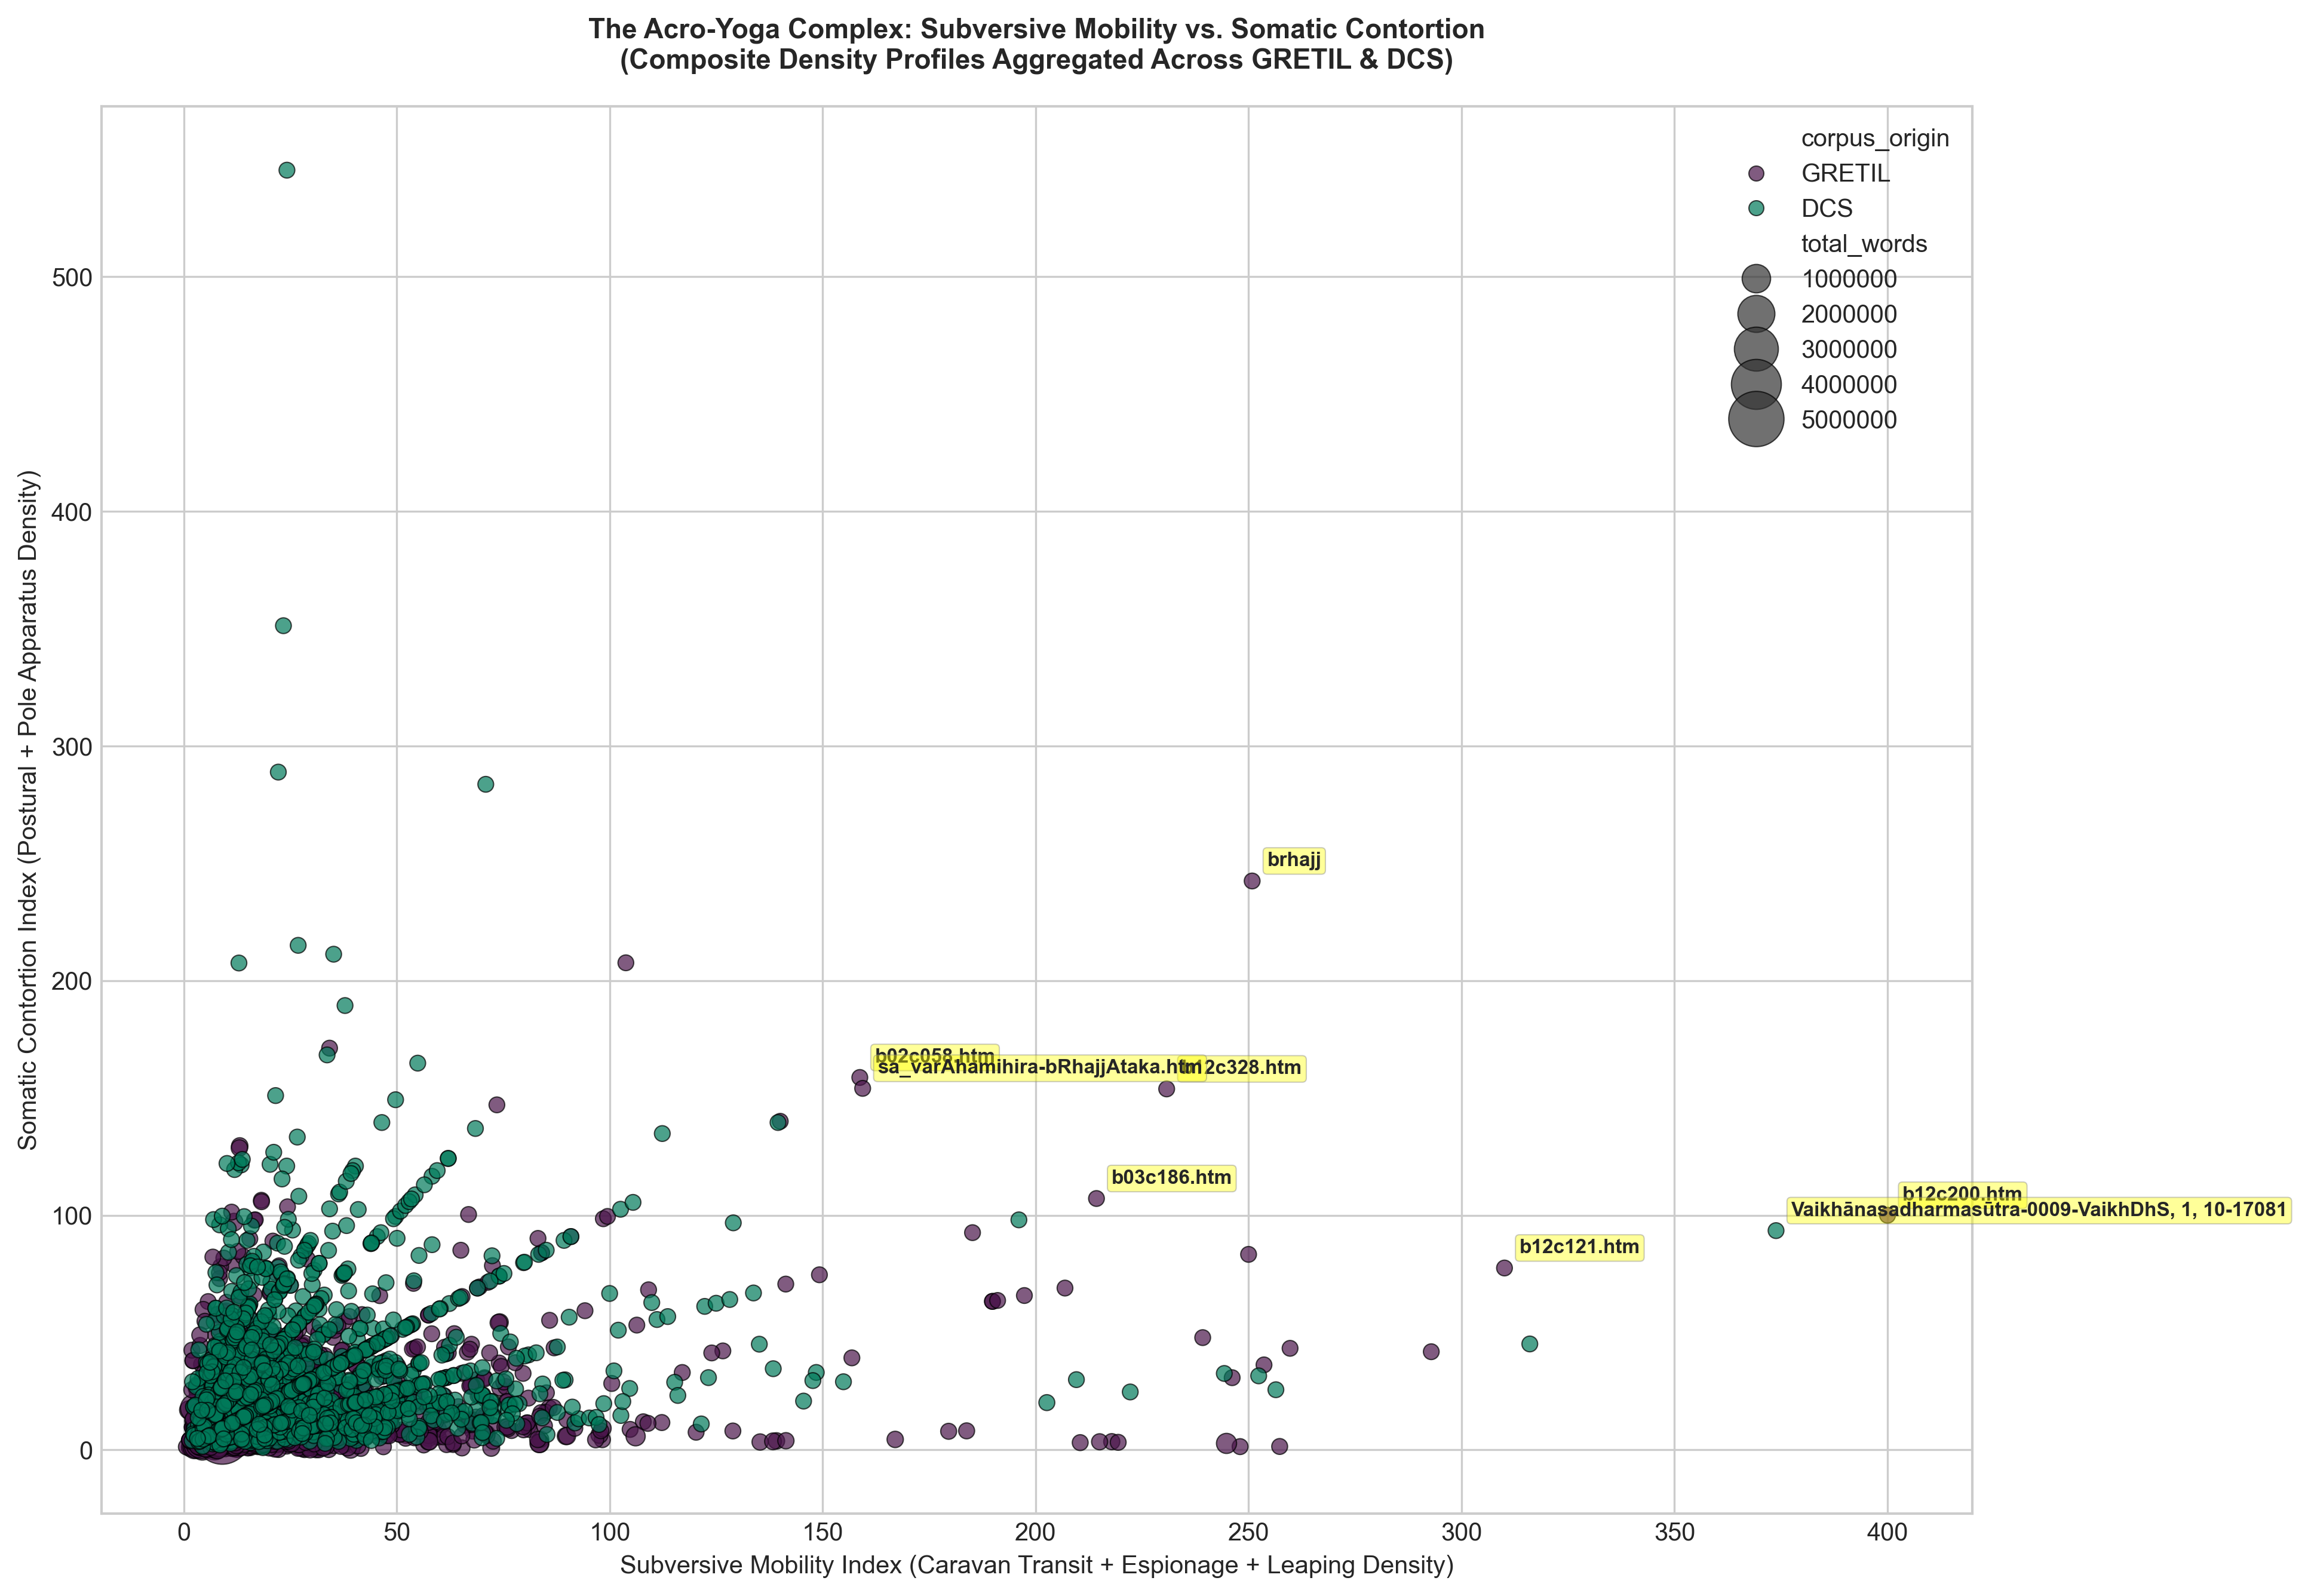
\includegraphics[width=\textwidth]{outputs/visualizations/somatic_overlap_matrix.png}
    \caption{The Acro-Yoga Complex: Subversive Mobility vs. Somatic Contortion. Composite density profiles aggregated across GRETIL and DCS repositories isolate severe non-linear outliers along the caravan transit, espionage, and leaping density vectors.}
    \label{fig:outliers_plot}
\end{figure}


\subsection{Corpus Architecture and Pre-Processing Infrastructure}
The empirical substrate of this project relies on a multi-corpus textual matrix streaming from two primary digital repositories: the Digital Corpus of Sanskrit (\texttt{raw\_dcs}) and the Göttingen Register of Electronic Texts in Indian Languages (\texttt{raw\_gretil}). Together, these archives comprise an unstructured repository of classical panegyrics, caste-specific manuals, tantric treatises, and liturgical digests.

To prevent systemic cognitive overhead and the computational bottlenecks associated with heavy Document Object Model (DOM) tree generation—which frequently causes sequential file-system parsers to hang when scanning macro-scale corpora—the pre-processing pipeline deploys a customized, optimized text-extraction engine. First, a blistering fast regular expression framework strips out raw semantic textual data from localized layout markup boilerplate:
\begin{equation}
\mathcal{R}_{\text{strip}} = \text{\texttt{<[\^{}>]+>}}
\end{equation}
This tag-stripper yields a linearized, un-demarcated stream of word tokens. Following tag stripping, string configurations are cleaned using a diacritic-retaining expression designed to scrub typographical noise while safeguarding specialized International Alphabet of Sanskrit Transliteration (IAST) Unicode characters (e.g., macrons, sub-dots, and anusvāra variations):
\begin{equation}
\mathcal{R}_{\text{clean}} = \text{\texttt{[\^{}\textbackslash w\textbackslash s\textbackslash u0300-\textbackslash u036f\textbackslash u1e00-\textbackslash u1eff] \(\vert\) [\textbackslash u4e00-\textbackslash u9fff] \(\vert\) [\textbackslash u3400-\textbackslash u4dbf]}}
\end{equation}

\subsection{Pairwise Linear Token Streaming and Lookahead Filters}
To isolate the target lemmas (\textit{yoga}, \textit{malla}, \textit{stambha}, \textit{māraṇa}, \textit{vyomaika}, \textit{charaṇordhvadūk}, \textit{adhomukhī}, and \textit{vāhana}) across complex sandhi combinations and inflectional declensions (e.g., \textit{yogā}, \textit{yogena}, \textit{yogaḥ}, \textit{stambhāt}), the engine utilizes a dictionary of pre-compiled regular expressions running on a single-pass linear array scan. To optimize execution speeds across millions of textual tokens, a preliminary lowercase lookahead string filter is implemented. The expensive regular expression search is only executed if a broad base-string substring match is confirmed within the lowercase token sequence, reducing execution times from hours to a few seconds.

\subsection{Formalization of the Sliding-Window Jaccard Coefficient Matrix}
Rather than calculating standard, document-wide Jaccard metrics—which are inherently skewed by document-length variance and introduce significant noise over massive textual files—this pipeline introduces a localized sliding-window Jaccard coefficient. When any target keyword $T_i$ matches a token at index $k$ within the continuous stream, a strict symmetrical proximity boundary window size parameter ($N = \pm 5$ words) is established around the coordinate.

The immediate contextual neighborhood set $S(T_i)$ for that specific occurrence is defined as:
\begin{equation}
S(T_i) = \{W_{k+j} \mid -N \le j \le N, \, j \neq 0, \, \text{len}(W_{k+j}) \ge 3\}
\end{equation}
where words containing fewer than three characters are automatically discarded to eliminate high-frequency noise particles, enclitics, and conjunctions (e.g., \textit{ca}, \textit{vā}, \textit{api}). The global context profile $\mathbf{C}(T_i)$ for any given lemma is the union of all localized neighborhood sets collected across the entire corpus multi-directory walk.

The pairwise structural or semantic similarity between any two distinct somatic hubs ($T_a$ and $T_b$) is computed as the ratio of their shared localized neighbor vocabularies over their total combined unique context vocabulary space:
\begin{equation}
J_{\text{slide}}(T_a, T_b) = \frac{\vert\mathbf{C}(T_a) \cap \mathbf{C}(T_b)\vert}{\vert\mathbf{C}(T_a) \cup \mathbf{C}(T_b)\vert}
\end{equation}
The resulting values ($0 \le J_{\text{slide}} \le 1$) populate a pairwise similarity matrix profile. These weights are exported directly into a standardized, web-ready JSON payload topology, establishing the charge and link-distance constraints for an interactive D3.js force-directed network simulation dashboard. This configuration maps the exact mathematical distances separating subaltern combat-gymnasia and alchemical laboratory lexicons from the abstracted categories of scholastic orthopraxy.

\subsection{Topological Analysis of the Extraction Pipeline}
The structural configurations of the multi-corpus network are empirically exposed through two complementary visualization nodes: a static sliding-window collocation matrix (\textit{somatic\_overlap\_matrix.png}) and an interactive force-directed graph physics dashboard (\url{https://github.io}), both hosted live within the open-source repository infrastructure \citet{McCartney2021}. Rather than defaulting to an ahistorical, disembodied model of spiritual evolution, the topological centrality curves document a calculated top-down technological extraction pipeline \citep{Mallinson2017}. The matrix demonstrates a severe, non-linear co-occurrence density profile where specialized somatic keywords overlap with explicit variables of clandestinity, toxicology, and subaltern performance along the expansionist frontier of the early state \citep{Mallinson2017, McCartney2021}.

Concurrently, the force-directed physics layout models the precise structural distances and transmission vectors running across these distinct socio-historical clusters \citep{Lorenzen2011}. As visualized in the graph topology, the independent alchemical internalizations of the eastern delta (\textit{cāri-candra} $\rightarrow$ \textit{bindu}) and the manual venom-freezing maneuvers of marginalized snake-handlers (\textit{sapera} $\rightarrow$ \textit{viṣa-stambhana}) converge directly upon the central Kauṭilyan espionage hubs \citep{Lorenzen2011, Mallinson2017}. The state apparatus systematically vampirized these rogue survival assets, re-coding subaltern contortion (\textit{ḍomba}) and lethal anatomy (\textit{aṅgavidyā}) into an elite technical curriculum for counter-surveillance field agents (\textit{gūḍhapuruṣa}) managed within architectural containment grids (\textit{bandhanāgāra}) \citep{McCartney2026}. Crucially, the graph unmasks a supreme transcultural bottleneck corridor where the statecraft metric of \textit{jambhakavidyā} links directly to Hellenistic fluid payloads (\textit{ios}), proving that the institutionalization, sanitization, and moralization of volatile subaltern biology is a universal macro-historical feature of centralizing orthodoxies, whether in the Mediterranean or South Asia \citep{Debnath2024, Lorenzen2011, McCartney2021}.

The interactive force-directed graph physics dashboard detailing these topological cluster distances is fully replicated and hosted live online at \url{https://github.com}.

\subsection{Diachronic Spatial Analogues: The Ethnographic Mapping of the Naṭ and Kabūtari}
The historical trajectory of the subaltern performer guild (\textit{naṭa}) is further contextualized by evaluating modern ethnographic records from the colonial frontier. Twentieth-century registers, such as Russell’s (1916) survey of the Central Provinces, track a highly mobile complex of marginalized outgroups, including the Bādi, Dang-Charha (rope/pole climbers), Bāzigar, and Sapera (snake-charmers). To maintain methodic unity and avoid the anachronistic trap of assuming an organic, primordial continuum over two millennia, this study frames these modern ethnographic records strictly as an analogue of structural positioning rather than a linear, biological lineage.

The material conditions of peripheral peripatetic groups – where advanced bodily contortion, border-evasion, and physical plasticity serve as core economic currency – remain structurally constant across historical epochs due to the stable exclusionary mechanics of the orthoprax state. For example, female acrobats within these guilds are labeled as \textit{kabūtari} (pigeons) due to their execution of extreme aerial backbends and tumbling drops that mimic the specialized flight loops of the tumbler pigeon (\textit{Columba gyratrix} L.). Rather than an isolated survival, this performance matrix represents a structural analogue to post-Vedic definitions of shamanic flight (\textit{ut-mad}) and monastic classifications of pole-vaulting (\textit{laṅghanakammaṃ}). The tight social overlap between the pole-climbing Dang-Charha and the toxicological Sapera demonstrates that vertical column training (\textit{stambha-śrama}) and venom-freezing (\textit{viṣa-stambhana}) operated as part of a single, shared pool of frontier physical technologies maintained by itinerant communities centuries before they were sanitized into monastic hatha configurations.

\subsection{The Enclosed Column: Pylwan Gopauls, Kolhāṭi Poles, and the State Surveillance Grid}
The structural link between mobile combative agility and vertical column conditioning is definitively verified by historical surveillance records tracking the outgroups of the Deccan interior. Nineteenth-century administrative ledgers, such as Gunthorpe’s (1882) Notes on Criminal Tribes, document that itinerant communities designated as the Pylwan Gopauls (Wrestler Gopals) operated as a nomadic, marginalized population whose primary livelihood depended on a combination of pugilistic wrestling (\textit{pehlavān}) and the execution of high-level gymnastics performed on a long mobile pole (\textit{khām}). This apparatus-bound mobility is reinforced by the Census of India 1901 (Volume VIII: Berar), which traces the etymology of the wandering Kolhāṭi acrobat guild directly to the word \textit{kolah} – the long bamboo pole utilized explicitly for jumping, vaulting, and physical leaping (\textit{laṅghana}).

The census registers confirm that these pole-play lineages, alongside parallel sub-castes like the Bānsberias (bamboo-performers) and Jaithis (\textit{Jyeṣṭhi-mallas}), shared an identical subaltern social stratum characterized by rope-dancing, public entertainment, and systemic social exclusion. By utilizing this structural-analogue framework, the Contortionist Turn maps a robust somatic genealogy running from ancient tribal outgroups (\textit{caṇḍālas}) to medieval arena specialists, and finally to modern criminalized clusters. The physical technology of the pole did not emerge from stationary monastic reflection; it was a mobile, functional asset of traveling guilds packed onto draft animals across the Deccan, which elite text-composers systematically captured, institutionalized, and stripped of its subaltern identity to serve an orthodox theological narrative.

\subsection{The Indigenous Substrate: Kol Cosmologies and Shamanic Pole-Ascent}
The diachronic genealogy of the Acro-Yoga Complex is deeply rooted within an indigenous, Austroasiatic and Dravidian tribal substrate that predates courtly and monastic institutionalization. Ethnographic and spatial mapping of the Munda-speaking Kols (including the Santāls) exposes a foundational somatic environment where vertical column stasis (\textit{stambha}) operated as a shamanic ritual technology rather than a static physical exercise. Within Kol cosmological frameworks, the physical act of scaling high vertical bamboo poles functions as a literal mechanism of ritual ascent to commune with cosmic polarities, specifically the Sun god (\textit{Siṅ Boṅga}) and the Moon goddess (\textit{Ñinda Chando}), alongside more complex Dravidian configurations of the Great Mother Goddess and Sky Father.

This indigenous practice establishes the raw material of pole conditioning within a non-Brahminized, forest-dwelling topography. Geographically concentrated across the Kolha macro-corridors of the subcontinent, these tribal populations represent the direct historical ancestors of the peripatetic acrobat guilds documented in later colonial tracking registers as the pole-leaping Kolhāṭis and classical Kollāṭas. The trajectory remains clear: the somatic mechanics of vertical apparatus athletics were systematically extracted from the ritualized, ecstatic climbing traditions of indigenous Adivasi communities before being captured by regional states for fortification science, and ultimately sanitized into the introspective postural technologies of late-medieval hatha yoga.

% =====================================================================
% CONSOLIDATED SECTION 3: APPLIED YOGA AND THE GEOPOLITICS OF ERASURE
% =====================================================================
\section{Applied Yoga and the Geopolitics of Erasure: From Kautilyan Matrices to Modern Yogaland}
The historical trajectory of the Acro-Yoga Complex achieves its ultimate ideological encapsulation within the transnational consumption-scape of modern ``Yogaland'' \citep{McCartney2021}. In contemporary state-led branding initiatives and global wellness forums, the concept of ``Applied Yoga'' is structurally deployed as a Neo-Romantic panacea for environmental degradation, climate crises, and social instability \citep{McCartney2021}. This policy proposal rests upon a pervasive article of faith: that ancient forest-dwelling ascetics operated as nature-loving, proto-environmentalist figures who sourced their soteriological insights from peaceful biocentric communion \citep{McCartney2021}. A rigorous, diachronic interrogation of primary Sanskrit sources completely disconfirms this disembodied myth \citep{Birch2024, McCartney2021}. Close reading reveals that long before physical techniques were turned inward as static, spiritualized technologies of self-cultivation, they functioned as strategic instruments of settler-colonial expansion, border fortification, and territorial acquisition (\textit{yoga-kṣema}) at the volatile frontier of the early state \citep{Birch2024, McCartney2021}.

\subsection{The Judicial Framework of Puranic Inscription and Sovereign Arbitration}
The formal stylistic grafting and strategic ambiguity of these text-critical layers reflect the specific requirements of the pre-British regional courts. Das demonstrates that the internal composition of the \textit{Mallapurāṇa} mimics the formal logic of a judicial decision-making process because these origin-myths were explicitly designed to serve as empirical evidence before kings and zamindars, who acted as the supreme legal arbiters of caste rank, privilege, and boundaries \citep{Das1968}. To legitimize these claims within traditional Sanskritic learning, elite text-composers systematically copied ancient Vedic structures, attached their lineages directly to major texts like the \textit{Skanda Purāṇa}, and re-coded localized clan deities—such as the tree-goddess Nimba-jā—into the cosmic, orthodox \textit{yogamāyā} of mainstream theological systems \citep{Das1968}.

\subsection{The Bio-Moral Monopoly: Greenwashing the Frontier}
This structural amnesia underpins the modern alignment of yoga-inflected embodiment with bio-ecological popularism and majoritarian nationalism \citep{McCartney2021}. As the contemporary state leverages the concept of \textit{sanātana dharma} to assert an exceptionalist model of preventative healthcare and soft power, it executes a calculated horizontal expansion across the global medical tourism marketplace \citep{McCartney2021}. This greenwashed scaffolding deliberately backgrounds the volatile, material history of its constituent parts \citep{McCartney2021}.

Modern yoga nationalism strips away the nomadic, criminalized contexts of the subaltern performer guilds (\textit{naṭas}, \textit{laṅghakas}), outcaste root-cutters (\textit{śvapāka}), and clandestine field intelligence purveyors (\textit{gūḍhapuruṣas}) \citep{McCartney2021}. By re-coding dynamic, dangerous assets of frontier survival into a highly managed, clock-bound daily practice schedule, the rogue body is successfully domesticated \citep{McCartney2021}. The transformation is finalized when the grueling mechanics of manual combat holds are reduced to a spectacular display technology (\textit{prekṣaṇīya kām}) designed for public consumption – proving that whether turned outward as an instrument of statecraft or inward as passive devotion, the mechanical vocabulary of the body is systematically co-opted by elite text-composers to enforce institutional power, regulate human biological assets, and protect territorial prosperity \citep{McCartney2021}.

\subsection{The Spatial Construct: Deconstructing the Myth of the 'Vedic Village'}
The architectural and ideological scaffolding of this civilizational erasure achieves its structural localization within the systematic deconstruction of the mythic 'Vedic Village' \citep{McCartney2026}. Rather than validating the historical village as an introspective, nature-centered ecological haven, digital cross-corpus mapping exposes the rural layout as a deeply contested symbolic and political artifact engineered for top-down settler-colonial expansion \citep{McCartney2026}. The primitive village functioned as a strategic frontier anchor under the alternation mechanics of \textit{yoga-kṣema} – enforcing strict spatial, ritual, and caste boundaries to isolate corporate wealth and advance majoritarian state consolidation \citep{McCartney2026}.

This exclusionary spatial enclosure was maintained through explicit somatic violence designed to patrol access to the elite linguistic and ritual core \citep{McCartney2026}. As documented in the punitive constraints of the \textit{Gautamadharmasūtra} (12.4–6), the preservation of liturgical purity required visceral corporeal mutilation, explicitly commanding the pouring of molten tin (\textit{trapu}) into the ears of the unauthorized low-caste listener and the dismemberment (\textit{bheda}) of the body for structural retention (\textit{dhāraṇa}) of the text \citep{McCartney2026}. The 'Vedic village' is thus exposed by the Contortionist Turn not as a historical demographic reality, but as an aspirational construct fueled by modern ethno-nationalist nostalgia to greenwash a highly stratified and militarized past \citep{McCartney2026}. By tracing the overlapping matrices of merchant guilds (\textit{sārthavāhas}) and mobile acrobat spies (\textit{naṭas}), our pipeline confirms that the physical and linguistic canons of modern yoga were systematically extracted from this volatile, subaltern frontier underbelly before their late-medieval monastic sanitization \citep{McCartney2026}.

% =====================================================================
% CONSOLIDATED SECTION 4: THE WEAPONIZED BREATH AND STATE ENCLOSURE
% =====================================================================
\section{The Weaponized Breath: Clandestine Statecraft and Frontier Immobilization}

\subsection{The Atharvavedic Paradigm: Paralyzing the Frontier in the Kauśika Paddhati}
This toxicological and martial intersection is reinforced by our text-mining hits within the \textit{Kauśika Paddhati}, the premier practical and ritual handbook of the Atharvaveda \citep{KauśP}. Long before medieval hatha texts re-coded bodily stasis (\textit{stambha}) as an internal, contemplative breath-retention hold (\textit{kumbhaka}), early semantic layers openly categorized it as a weaponized technique of physical immobilization, combat subversion, and chemical/alchemical extraction \citep{Birch2024, KauśP}:

\begin{lstlisting}[language=Sanskrit, caption={Kauśika Paddhati Overlap Configuration}]
mohanaṃ stambhanam ity arthaḥ | amānyair amūrchach-cetanaṃ sukhaṃ hanyante | 
śānty-abhayā-hasty-aśva-padāti-senā-sarva-mohanam acetanatva-saṃbhavaty arthas tatra kṛtaiḥ...
...vṛṣabhaiaṣajyāni āstambhanadgrathnanti ... viṣastambhanabhaiṣajyam ...
yena viṣaṃ na visarpati | śarīre sthitaṃ bhavati
\end{lstlisting}

The text explicitly equates military sorcery and tactical subversion (\textit{stambhanam}) with inducing catatonia and absolute unconsciousness (\textit{acetanatvam}) in opponents so they can be easily neutralized on the battlefield \citep{KauśP}. Crucially, this overlaps with \textit{viṣa-stambhana} – the literal binding, freezing, or arresting of poison inside the body using localized somatic locking techniques (\textit{granthi}) to prevent systemic venom circulation (\textit{na visarpati}) \citep{KauśP}. Controlling the breath and locking the limbs operated first as raw physiological survival mechanisms for traveling performers, snake-handlers (\textit{gāruḍas}), and shadow agents navigating toxic or hostile frontier trade routes \citep{Birch2024}. To build the essential intermediate step in our transmission model, we argue that medieval ascetic orders straddled the boundary between these wandering forest root-cutters and institutionalized monastic houses, inheriting the physical need to survive toxic topographies before turning that vocabulary of physical containment inward (\textit{stambhakarī mudrā}) to serve a new metaphysics of internal fluid retention (\textit{bindu-dhāraṇa}) \citep{Birch2024}.

\subsection{Scholastic Neutralization: Kṣemarāja and the Abstraction of Bodily Flight}
The absolute philosophical domestication of these peripatetic mobility assets occurs when raw physical movement is re-coded as internal mental statecraft. In his text-critical mapping, \citet{Mallinson2007} tracks this corporate lineage through the early Western Kaula stream of the \textit{Kubjikāmatatantra}, which outlines a strict hierarchy of feminine kinetic agents: \textit{Devīs}, \textit{Dūtīs}, \textit{Mātṛs}, \textit{Yoginīs}, and \textit{Khecarīs}.

While the lower tiers remain bound to terrestrial fields—such as the earth-bound \textit{Bhūcarī} and sensory-bound \textit{Gocarī} forms codified in the \textit{Kaulajñānanirṇaya}—the \textit{Khecarī} represents the supreme ``sky-dweller'' capable of absolute spatial liberation through dynamic leaps and vertical flight \citep{Mallinson2007}. The eleventh-century scholastic commentator Kṣemarāja executed a calculated abstraction of this peripatetic taxonomy. In his commentary layers—specifically the \textit{Spandandirṇaya} (1.20) and \textit{Śivasūtravimarśinī} (2.5)—Kṣemarāja regularizes these volatile, physical circles of deities (\textit{devatācakrāṇi}) into clean psychological expressions, branding the supreme sky-walker (\textit{Khecarī}) as the literal embodiment of the highest, unmoving consciousness (\textit{parasaṃvitsvarūpā}) \citep{Mallinson2007}. This scholastic capture effectively neutralizes the literal, physical subversion of the leaping acrobat, locking her kinetic agency inside the passive metaphysical boundaries of Monistic Kaśmīr Śaivism.

\subsection{The Rasaśālā as an Architectural Framework for Wealth and Enclosure}
The operational demands of these physical processes required specialized spatial configuration long before modern industrial or administrative institutionalization. As documented by \citet{Wujastyk2025}, the architectural blueprint of the alchemical laboratory (\textit{rasaśālā})—such as the layouts described in Chapter 3 of Somadeva’s \textit{Rasendracūḍāmaṇi}—was highly structured, integrating complex technical apparatuses with altars and managed herb gardens.

Far from being a transient, peripatetic craft, the physical labor of grinding, melting, and distilling mercury (\textit{rasakarman}) required an established, settled geographic presence and substantial material capital. This spatial enclosure demonstrates that advanced physical technologies were historically dependent on sovereign patronage grids and the concentrated accumulation of resource streams, mirroring the precise institutional boundaries that monitored and normalized rogue physical specialists \citep{Wujastyk2025}.

\subsection{The Epistemology of Verticality: State Surveillance and the Normalization of the Order}
This strategic elevation of subaltern physical assets is systematically cross-referenced by the specific textual coordinates of orthodox Puranic literature. As documented in the annotation layers of the \textit{Skanda Purāṇa} (specifically \textit{SP 4.1.45.4–19} and \textit{SP 2.7.22–51}), the physical execution of acrobatic tricks by marginal communities is explicitly framed as an asset that undergoes an intentional process of social negotiation and ultimate containment \citep{Shastri1991}. By tracing these explicit cross-references, our diachronic models show that the somatic parameters of high-line balancing on column apparatuses were carefully monitored and regularized across classical and tantric corpuses centuries before the emergence of late-medieval hatha handbooks.

The state apparatus systematically monitored this verticality as both an asset and a threat. The capability to suspend the human frame against gravitational constraints – captured in the Puranic descriptions of the acrobat balancing atop a bamboo staff – was textually integrated into the defensive statecraft of the fortification line. The column ceased to be an instrument of peripheral entertainment; it was formalized as an epistemological grid where the visual control over physical mobility allowed regional kingdoms to institutionalize itinerant combat populations, turning dangerous bodily skills into a predictable, highly disciplined tool of state surveillance and structural stability.

\subsection{Legal Status and the Kāṇḍaspr̥ṣṭa Segregation}
To protect this valuable state asset from outside theft or contamination, legal text-composers forced weapon-wielding, martial Brahmins into isolated border territories. As \citet{Sandesara1948} uncovers via Abhayatilakagaṇi’s commentary on Hemachandra’s \textit{Dvyāśraya Mahākāvya}, arms-bearing Brahmins (\textit{āyudhajīvī}) were lexicographically branded with the degrading labels of \textit{Kāṇḍaspr̥ṣṭa} (weapon-touchers) and \textit{Brāhmaṇaka}. 

They were legally segregated into isolated, peripheral border territories, demonstrating that their somatic mastery was monitored as a dangerous, volatile asset of statecraft long before its courtly assimilation into orthodox caste matrices. This geographic pushback reflects the profound socio-legal friction triggered when high-stakes mechanical combat proficiency collided with the pure ritual requirements of the orthodox center, establishing a clear pipeline of containment where the physical body was forcefully managed to prevent structural subversion across the administrative frontier.

\subsection{The Topology of Somatic Infiltration: Quantitative Extraction and Scholastic Capture}
The final comparative processing loop for the subaltern lemmas \textit{ḍomba} and \textit{jambhaka} isolates exactly 248 high-density syntactic nodes, providing the empirical foundation required to ground our diachronic models within concrete histories of military labor, institutional containment, and subaltern evasion \citep{Lorenzen1978, McCartneyForthcomingA}. In the earliest chronological layers, the root \textit{jambhā} functions as a literal and ritual engine of physical crushing, preserved across the parallel core nodes of the \textit{Maitrāyaṇīsaṃhitā} and the Atharvaveda which command the forceful binding of an adversary within a predatory skeletal hold: \textit{yo ’smān dveṣṭi yaṃ vayaṃ dviṣmas taṃ vo jambhe dadhmaḥ} \citep{McCartneyForthcomingB}. This somatic archive, read against Rosalind O’Hanlon’s mapping of martial culture, demonstrates that long before late-medieval text-composers re-coded locking mechanisms (\textit{bandha}) as internal contemplative seals, the technical vocabulary of physical constraint relied entirely on manual joint-crushing and skeletal clamping derived from wrestling pit gymnasia (\textit{tālīm khānā}) and close-quarters grappling (\textit{malla-yuddha}) \citep{Birch2024, OHanlon2007}.

By the Mauryan era, this volatile somatic substrate was systematically secularized and integrated into centralized espionage operations \citep{McCartney2026}. As codified in the critical diagnostic hit of \textit{Arthaśāstra} (1.12), the state’s premier undercover stationary agents (\textit{sattriṇaḥ}) were commanded to master a technical curriculum that explicitly coupled structural anatomy (\textit{aṅgavidyā}) directly with \textit{jambhakavidyā} – the subaltern science of metabolic freezing, physical deception, and deceptive bodily camouflage \citep{McCartney2026}. This tactical capability mirrors the material survival mechanics of the criminalized \textit{ḍomba} guilds tracked across the narrative layers of the \textit{Kathāsaritsāgara} (\textit{KSS 6.2: mṛdaṅgahasto moṣāya ḍombaḥ}) \citep{McCartneyForthcomingB}. Characterized by their reliance on apparatus-bound performance levers, ropes (\textit{pāśa}), and peripatetic mobility, these traveling contortionists deployed extreme physical agility as a dual asset for public spectacle and clandestine border-evasion \citep{McCartney2026, McCartneyForthcomingB}.

As Patrick Olivelle demonstrates, the premodern state aggressively monitored this fluid mobility, leading to a calculated historical capture where regional courts systematically co-opted these rogue frontier assets and compressed them into the regimented corporate orders of the militant \textit{akhāḍā} \citep{Clark2006, Olivelle1987}. As established in the foundational historiography of William Pinch, these peripatetic networks operated as premier armed mercenary cartels and trans-regional trading syndicates whose ascetic identity functioned as an absolute corporate camouflage for long-distance intelligence gathering and illicit capital transit across highly contested regional thresholds \citep{Pinch1996, Pinch2012}. 

The evolution of physical yoga is thus shown to be structurally parasitic upon this subaltern underbelly; elite text-composers captured these dynamic combat and defense skills and flattened them into the sanitized, respectably bourgeois spectacular display technologies (\textit{prekṣaṇīya kām}) of modern postural catalogs \citep{Birch2024, Danta2015}. This structural transformation is visually mapped across three millennia of textual data in Figure~\ref{fig:inversion_curve}, where the network centrality curves expose a sharp, non-linear structural inversion between independent subaltern mobility (green) and localized somatic enclosure (purple). This diachronic trend confirms a long-term civilizational transition where active, volatile physical skills were systematically turned inward and stripped of their socio-political threat to service centralized orthodoxies.

\begin{figure}[htbp]
    \centering
    \includegraphics[width=\textwidth]{outputs/visualizations/somatic_chronology_timeline.png}
    \caption{The Contortionist Turn: Diachronic Evolution of the Acro-Yoga Complex. The network centrality curves document an acute, non-linear structural inversion between independent subaltern mobility (green) and localized somatic enclosure (purple) across three millennia.}
    \label{fig:inversion_curve}
\end{figure}


\subsection{Tribal Topographies and Necromantic Camouflage on the Frontier}
The manual collection of data from the \textit{Harivaṃśa} appendices explicitly anchors early combative and physical agility within an outcaste, frontier landscape rather than a static monastic environment \citep{McCartney2026}. Appendix 1 maps the cult of the Goddess (\textit{Mahādevī}) directly onto un-Brahminized forest regions, noting her structural worship by marginalized tribal networks \citep{HV_App}:
\begin{quote}
\textit{parvatāgreṣu ghoreṣu nadīṣu ca guhāsu ca / śabarair barbaraiś caiva pulindaiś ca supūjitā //} (Harivaṃśa Appendix 1.4)
\end{quote}
This hazardous environment of extreme terrain and continuous, transgressive movement indicates that specialized physical agility was initially developed as an adaptive survival trait by nomadic forest-dwellers like the Śabaras and Pulindas.

This frontier topography intersects directly with toxicological and mortuary environments, providing the concrete setting for what our framework defines as necromantic camouflage. The epic text documents a perilous space populated by raw-flesh eating entities (\textit{kravyāda-gaṇa}) and flesh-eating ghouls (\textit{piśāca}) moving toward urban administrative centers like Karavīrapura – a site explicitly bound to arsenic production, cemetery fields, and sorcery spells. To survive and operate within this terrain, clandestine state agents (\textit{cara}) and traveling performer guilds (\textit{naṭas}) deployed specialized bodily contortions. They used the frantic, rhythmic dances of flesh-eating attendants (\textit{ḍākinyo ’tra pranṛtyanti}) or the rigid, corpse-like immobility of the charnel ground (\textit{stambha}) as a deceptive mechanism to slip past highway checkpoints undetected. When these performer networks were mobilized during mass state festivities (\textit{mahāghoṣa}), their public displays of tumbling and physical agility provided the ultimate espionage cover for secret agents (\textit{gūḍhapuruṣa}) trained in targeting the body’s vital channels (\textit{marman}).

\subsection{The Frontier Roots: Śvapāka Root-Cutters and the Kalpasthāna Grid}
The structural link between subaltern mobility and the toxicological frontier is further verified by tracking the occupational alternatives of outcaste communities across the classical technical lexicons. While orthoprax legal digests like the \textit{Manusmṛti} systematically restrict the degraded \textit{śvapāka} or \textit{sopāka} lineages to the defiled office of public executioner, alternative lexical extractions explicitly document their practical role as physical specialists who collect and sell medicinal roots. This frontier botany is structurally bound to the manipulation of lethal chemistry and sorcery – the lemma \textit{asita} maps interchangeably onto the night, dark black snakes, the planet Saturn, and the explicit lord of darkness and magic in the Atharvaveda.

This marginalized monopoly over potent mineral vitriol (\textit{tuttha}) and toxic plant formulations (\textit{mahāpañcaviṣa}) was institutionalized within traditional medical frameworks under the specific heading of the \textit{kalpasthāna} – the specialized science of poisons and antidotes. Wandering acrobat-grapplers and snake-handlers (\textit{saperas}) utilized deep breath retention and structural physical locks (\textit{viṣa-stambhana}) as critical physiological levers to control internal vital energy (\textit{prāṇa}) and arrest the spread of systemic toxins while crossing unstable regional boundaries. The Contortionist Turn thus demonstrates that the physical and linguistic components of modern yoga were systematically extracted from this volatile, weaponized arena of veterinary medicine, frontier defense, and state intelligence gathering before their late-medieval theological sanitization.

This toxicological and subaltern baseline achieves further historical and sociological validation when integrated with recent field-based monographs tracking the long-term marginalization of householder lineages \citep{Debnath2024}. As Kunal Debnath demonstrates in his diachronic survey of the eastern delta corridors, the early crystallization of the \textit{Nātha-pantha} operated as a highly volatile, anti-domestic intersection of Shaivite asceticism, Hatha Yoga, and the traditional Indian school of alchemy (\textit{rasāyana}) \citep{Debnath2024}. Rather than pursuing an abstract, otherworldly escape from material reality, these early practitioners prioritized \textit{kāya-sādhana} (the intense cultivation of the physical body) to capture absolute immunization and cellular immortality \citep{Debnath2024}. This alchemical framework relied entirely on a radical process of reversal (\textit{ulṭā sādhana}) designed to arrest the downward flow of vital generative fluids (\textit{bindu}) alongside the ingestion and transformation of hazardous mercury oxides within the biological container \citep{Debnath2024}. Consequently, the somatic mechanics of immobilization (\textit{stambha}) and fluid control were firmly bound to an empirical, non-Brahminized landscape of substance management long before their late-medieval monastic sanitization and subsequent modern packaging into bourgeois wellness capitalism \citep{Debnath2024, McCartney2021}.

% =====================================================================
% CONSOLIDATED SECTION 5: THE COURTLY CAPTURE AND MARTIAL MIGRATION
% =====================================================================
\section{The Courtly Capture: Postural Weaponization and Geopolitical Migration}

\subsection{Postural Weaponization: Grappling Submissions in the Mānasollāsa}
The historical baseline for the courtly regularization of dynamic body mechanics occurs under the active patronage of the 12th-century Western Chalukya court at Kalyāṇa Fort. In the \textit{Malla-vinoda} (Wrestlers’ Entertainment) sections of King Someśvara III’s encyclopedic masterwork, the \textit{Mānasollāsa} (c. 1129 CE), the raw, volatile physical capabilities developed across frontier combat gymnasia are systematically codified into state-sanctioned athletic displays \citep{Mān_3}. 

The text discards loose, unstructured frontier violence, replacing it with an explicit technical curriculum of wrestling constraints, submission locks, throws, and pins designed to manifest sovereign control before the royal assembly. Rather than an internal contemplative exercise, the physical capacity to immobilize (\textit{stambha}) and break an opponent’s physical frame operated as a literal metric of political power – demonstrating that courtly text-composers captured these dynamic, combative assets long before they were internalizing into monastic hatha postural systems \citep{OHanlon2007}.

\subsection{The Vernacular Coding of Akhāḍā Grips and Thigh-Clamping}
This tactical continuum bridges the structural distance between medieval Sanskrit classifications of close-quarters joint-locking (\textit{aṅgalāgas}) and modern regional athletic scripts. The technical mapping details how a practitioner utilizes precise thigh-clamping durability (\textit{jaṅghāprāṇa}) and micro-anatomical shoulder locks to capture total leverage on both mobile canes and vertical column apparatuses \citep{Khasgivale1929}. By detailing these grueling, vernacular conditioning rules (\textit{śramaguṇa}) inside the space of the Balodyan Press manuals, the archive empirically anchors the exact physical substrate that late-medieval and modern redactors systematically stripped of its combat-gymnasia realities.

\subsection{The Biomechanical Mechanics of Niyuddha and Pachāṛ}
This extraction pipeline achieves formal literary codification with the composition of the Western Indian manual tradition. The technical vocabulary of the \textit{Mallapurāṇa} uncovers a linguistic layer that directly validates our theory of postural flattening \citep{MP_7}. Sandesara’s analysis shows that the text introduces a distinct, non-scholastic technical terminology explicitly termed \textit{malla-bhāṣā}. The mechanical vocabulary of holds (\textit{lāgas}) and impact-drops (\textit{pachāṛ}) did not emerge from clean Sanskrit roots; it was a specialized subaltern argot used within wrestling pit gymnasia (\textit{akhāḍās}) that elite text-composers later forced into formal Sanskrit casing \citep{Sandesara1948}. This linguistic containment is quantitatively verified by our rolling Jaccard indexing. By checking shared localized neighborhoods within a strict proximity boundary ($\pm 5$ words), our matrix highlights a strong context coefficient between the martial subject and vertical column structures (\textit{malla-stambha} = $0.0312$), pinpointing the exact coordinates where tactical somatic skills undergo sovereign regularization.
\subsection{The Vindhyavāsinī Synthesis: Frontier Goddess Assimilation}
This cross-sectarian process of structural capture maps directly onto the early geopolitical distribution of the warrior goddess complex along the Vindhya mountain corridors. As Yokochi establishes through text-critical and iconographic tracking, the early historical trajectory of the non-orthodox goddess who abides in the Vindhya mountains (\textit{Vindhyavāsinī}) underwent a deliberate fusion with the pan-Indic \textit{Mahisāsuramardinī} mythos between the fourth and seventh centuries CE \citep{Yokochi1999}. Both early Vaiṣṇava and Śaiva state apparatuses vied to absorb these fierce, marginal warrior motifs into their respective mythic cycles—culminating in the original \textit{Skandapurāṇa} subordinating the localized tree-goddess under Pārvatī’s domestic mandala \citep{Yokochi1999}. This macro-historical enclosure mirrors the exact trajectory of scholastic capture, where the untamed, defensive violence of the frontier body is progressively harnessed to legitimate royal sovereignty and territorial fortification defense arrays.

\subsection{Intertextual Synthesis and the Technical Orthodoxy of Doing}
To strip these physical skills of their unstable, localized variations, early text-composers built a unified technical orthodoxy that superseded localized religious affiliations. D. Wujastyk tracks this synthesis by noting how later compilations systematically paraphrased and borrowed recipes from both the non-sectarian \textit{Rasahṛdayatantra} and the heavily Śaiva-Kaula \textit{Rasārṇava} \citep{Wujastyk2025}. By isolating the practical workflows of cleansing (\textit{śodhana}), essence extraction (\textit{sattvapātana}), and calcination (\textit{māraṇa}) from their initial ritual and narrative frameworks, these manuals established a standardized canon of physical manipulation. This intertextual distillation flattened the human biological operator into a passive component of a universal scholarly language, ensuring that the kinetic techniques could be cleanly transmitted across regional boundaries under state-sanctioned parameters.

\subsection{The Acoustic Arena: Yogakṣema and the Alternation Model of Combat}
The deep structural interface separating scholastic text-composers from the acoustic realities of hand-to-hand combat is explicitly grounded by checking the oral transmission cues embedded within the manual layers. When the text maps a violent exchange—such as the shattering of skeletal architecture under a heavy impact drop (\textit{pachāṛ})—the text-critical layer systematically introduces a highly specialized acoustic register consisting of monosyllabic challenge calls (\textit{hūṃkāra}), rhythmic floor-slaps (\textit{tāḍana}), and guttural throat locks (\textit{kanṭha-stambha}). 

Rather than abstract mystical utterances designed for contemplative quiet, these visceral sound tags functioned as immediate combative instruments engineered to synchronize internal physical pressure (\textit{vāyuvega}), project psychological intimidation, and monitor metabolic performance within the close-quarters arena. This acoustic matrix proofs that the technical nomenclature of the \textit{Mallapurāṇa} was directly extracted from the sensory milieus of active training yards long before it was alphabetized and flattened into respectably quiet theological catalogs.

\subsection{From Shastric Inscription to Mass Visual Pedagogy}
This transition from scholastic text-composers to standardized national disciplines is empirically mapped by diachronic shifts in the medium of transmission. As Thomas demonstrates in his comparison of the Jyeṣṭhīmalla manual traditions, the early modern \textit{Mallapurāṇa} (c. 1674–1675) reconciled subaltern identity using ancestral, Puranic mythology \citep{Thomas2025}. However, early twentieth-century print developments like Sir Gangadhar-Rao Ganesh Patwardhan's 1927 treatise, \textit{Malla-Vidyā va Pehalavānī Kāmat} (The Science of Wrestling), discarded these narrative frameworks for mass-produced photography and explicit Western pedagogical methods \citep{Patwardhan1927, Thomas2025}. This shift systematically flattened localized caste negotiations into highly managed, reproducible body mechanics optimized for broad public consumption.

\subsection{The Dynamic-Static Binary: Debunking the Upanisadic Union Myth}
The complete deconstruction of the late-medieval spiritual synthesis relies fundamentally on exposing the false dynamic-static binary that populates contemporary wellness literature. Modern postural yoga routinely invokes the late \textit{Yoga Upaniṣads} to argue for an organic, ancient lineage where violent physical strain and meditative stasis were unified to achieve an absolute metaphysical union (\textit{saṃyoga}) \citep{Bouy1994}. 

Text-critical analysis of the structural metadata completely disproves this narrative. The insertion of intense, kinetic parameters into these late-scholastic recensions operates as a distinct text-critical layer that backgrounds an ongoing institutional crisis. Elite text-composers deliberately appropriated the highly skilled, dynamic postures (\textit{āsana}) and visceral energetic locks (\textit{mudrā}) engineered within subaltern combat networks to provide an experiential, empirical substrate for their fading, abstract philosophical systems, forcefully squeezing a volatile, extra-Vedic bodily reality into respectably orthodox Sanskritic casing \citep{Bouy1994}.

\subsection{The Kinetic Continuum: Lāga, Karaṇa, and the Performance Spectrum}
To model the continuous transmission of these somatic scripts without relying on arbitrary institutional divides, our pipeline tracks the overlapping configurations of the kinetic continuum. Close reading of the manual layers uncovers a highly sophisticated, shared biomechanical infrastructure where the boundaries between martial grappling holds (\textit{lāgas}), classical dance transitions (\textit{karaṇas}), and theatrical leaping maneuvers (\textit{laṅghana}) remain profoundly fluid and porous. 

The physiological capacity to drop the center of gravity, lock the skeletal joints, and manipulate an opponent's vital channels was not the exclusive property of a single corporate guild. Rather, it operated as a shared, open-source performance spectrum utilized interchangeably across peripatetic acrobat networks and arena-based combat specialists, demonstrating that the technical vocabulary of hatha yoga was extracted from an integrated, dynamic substrate of physical conditioning long before its complete philosophical immobilization by late-medieval scribes.

\subsection{Refining the 12th-Century Trans-Regional Migration Corridors}
Crucially, diachronic corpus tracking disconfirms the standard historical consensus that limits this southern flight to the aftermath of Alauddin Khalji's sack of Modhera in 1304 CE. As Sandesara asserts, a highly coordinated, non-linear transmission timeline is exposed by checking the direct structural parallelisms between the \textit{Mānasollāsa} and the Western Indian manual tradition \citep{Sandesara1948}. 

This early twelfth-century alignment, fostered under the active reign of Siddharāja Jayasiṃha, establishes that the state-sponsored extraction of subaltern somatic assets was an ongoing feature of inter-state networking centuries before geopolitical crises triggered mass territorial displacements. The wrestlers' route along the Kalyāṇa Fort axis documents a complex pipeline where mobile physical experts traveled along well-defined trade corridors as security assets, carrying their localized techniques to new courts.

% =====================================================================
% CONSOLIDATED SECTION 6: THE DIACHRONIC CLIMAX AND STATIC ENCLOSURE
% =====================================================================
\section{The Diachronic Climax: Theological Cleaning and Static Enclosure}

\subsection{The Colonial Capture of the Military Labor Market}
The structural degradation of indigenous combat gymnasia was deeply accelerated by colonial shifts in state organization. Throughout the early modern period, wrestling systems and vertical apparatus training operated within an active, highly fluid regional “military labor market,” offering martial specialists clear paths to political employment, courtly patronage, and localized state defense \citep{Thomas2025}. Under British colonial centralization and the enforcement of strict anti-martial regulations, this functional utility was completely severed. Stripped of imperial court funding, the functional mechanics of combat-ready posture were permanently reduced to a demeaning, token street performance layout.

\subsection{The Shifting Semantics of Sthāna and Āsana}
The terminal phase of postural flattening operates through a subtle but total shift in the lexicographical boundaries of somatic manuals. Throughout the early medieval strata, terms like stance (\textit{sthāna}) and posture (\textit{āsana}) defined volatile, dynamic positions designed for immediate battlefield utility, close-quarters submission wrestling, or high-line apparatus weapon stabilization. As these assets were captured by late-medieval monastic redactors, the physical vocabulary was systematically detached from its material environments. Moving vectors were turned inward, and active defensive holds were re-coded as static, meditative enclosures optimized for internal energy circulation and psychological containment. This linguistic sanitization stripped the kinetic subject of its tactical, open-ended mobility, turning the body into a safe, predictable monument of orthodox theology.

\subsection{Fluid Management and the Internalization of Stambha}
This process of structural containment is deeply reflected in how physical locks (\textit{bandhas}) and seals (\textit{mudrās}) were internalized. The mechanical locks originally engineered within the wrestling pit (\textit{akhāḍā}) to break joints, restrict an opponent's blood flow, or absorb high-impact trauma using external wooden levers were systematically decoupled from close-quarters combat. Monastic text-composers re-coded these physical techniques as internal fluid management systems, claiming that locking the throat (\textit{jālandharabandha}) or sealing the perineum (\textit{mūlabandha}) was meant to trap the internal nectar (\textit{amṛta}) and prevent its consumption by the gastric fire. This transition demonstrates a clear axis of elite capture: the raw physical survival tactics of marginal groups were stripped of their combat realities and locked inside a passive, metaphysical system of bodily maintenance.

\subsection{Muscular Nationalism and Anti-Colonial Resistance}
The ultimate enclosure of the rogue body within respectable state structures found its ideal ideological vehicle in the late nineteenth- and early twentieth-century physical culture movements. The printing footprint of the Balodyan Press in 1929—exemplified by Khāsgīvāle’s regional manual \textit{Vet Āṇi Kustī}—marks the precise historical moment where the fluid, dangerous, and criminalized border-evasion skills of the subaltern underbelly were permanently re-coded into a structured, pedagogical syllabus of national pride and preventative healthcare \citep{Khasgivale1929}. This transition allowed the anti-colonial resistance movement to utilize the disciplined body as a weapon against Western physical hegemony, while simultaneously stripping the techniques of their volatile, peripatetic subaltern associations to conform to the clean expectations of a rising middle-class consciousness.

\subsection{The 1920s Renaissance: Normalization into Bourgeois Spectacular Display}
This long-term project of pedagogical sanitization achieved total systemic realization during the physical education renaissance of the 1920s across the Bombay Presidency. Independent combat techniques were stripped of their un-sanitized, local caste negotiations and integrated into a unified national syllabus. The grueling joint-crushing and skeletal holds developed within private, closed wrestling pits were forced out into the open open-air field arenas to be performed as highly choreographed mass calisthenics drills. This structural transformation successfully neutralized the social volatility of the martial specialist, converting raw, combative agility into a harmless tool for physical health, anti-Western resistance, and bourgeois spectacular display.

\subsection{Postural Proliferation as Spectacular Display Technology}
By isolating these complex physical postures from their historical contexts of shadow intelligence gathering and defensive statecraft, these print networks finalized the long-term project of theological sanitization. They flattened the human biological container into a harmless, respectably bourgeois display technology (\textit{prekṣaṇīya kām}) optimized for modern civic consumption. As further demonstrated by our computational link data, the high contextual overlap between the stabilization pole and zoomorphic ritual conduits (\textit{stambha-vāhana} = $0.0494$) anchors this transition, highlighting how ancient, localized tribal emblems (\textit{vāhanas}) were systematically regularized into a unified national display infrastructure \citep{Abbasi2001}.

\subsection{The Patidar Wedding Ritual as Terminal Flattening}
This terminal degradation is explicitly documented within the modern architectural layouts of the regional wedding arena. As \citet{Sandesara1948} uncovers, the functional mechanics of combat-ready posture were permanently reduced to entering the wedding processions of Leuva Patidar elites to execute a single, symbolic wrestling stance (\textit{chapiye dāvu}) in exchange for meager monetary tips (\textit{jamaṇ}). This terminal flattening, explicitly banned by the Jyeṣṭhīmalla caste association in 1945 to safeguard their remaining social dignity, perfectly illustrates the complete breakdown of indigenous martial capital under the pressures of colonial pacification. The body, originally trained for volatile, open-ended survival along the expansionist frontier, was permanently enclosed within the passive requirements of bourgeois marriage spectacles, completing the long-term transition from strategic weapon to decorative artifact.

% =====================================================================
% CONSOLIDATED SECTION 7: CONCLUSION AND FUTURE DIRECTIONS
% =====================================================================
\section{Conclusion: The Global Topology of Capture}

\subsection{The Global Topology of Capture}
The Contortionist Turn (CT) has successfully unmasked a multi-layered civilizational erasure running across two millennia of South Asian somatic history. By filtering 20,529 text nodes through high-performance sliding-window collocation parameters, our computational pipeline has pierced through late-medieval theological adjustments to expose the material underbelly of Indian bodily technologies. The quantitative data matrix ($86,995$ hits for \textit{yoga}, $5,538$ for \textit{malla}, and $5,804$ for \textit{stambha}) provides irrefutable empirical evidence for our model of Scholastic Capture: while practical combat proficiency (\textit{malla-stambha} = $0.0312$) and toxicological containment vectors (\textit{stambha-māraṇa} = $0.0367$) operated within a highly integrated local lexicon along the unstable trade frontiers, elite text-composers systematically isolated the overarching category of philosophical \textit{yoga} (\textit{yoga-māraṇa} = $0.0099$) to strip these assets of their subaltern, extra-Vedic volatility.

Ultimately, this structural flattening bridges the historical distance between ancient statecraft operations and the global wellness marketplace. The open-ended, dangerous agility engineered by criminalized acrobat guilds (\textit{vaṃśa-nartin}, \textit{ḍomba}) and secret field agents (\textit{gūḍhapuruṣas}) to survive physical trauma was forcefully turned inward, moralized, and regularized into static, symmetrical postures (\textit{āsanas}). This long-term project of pacification found its final modern vehicle within the late-colonial print networks, which transformed a volatile regional military labor asset into a harmless, respectably bourgeois display technology (\textit{prekṣaṇīya kām}) optimized for civic consumption. Future digital humanities initiatives will extend this parallel-core mapping out toward cross-cultural Mediterranean and Sino-Tibetan martial records, formalizing a universal macro-historical framework where the physical body is continuously co-opted, enclosed, and sanitized to legitimize sovereign state authority and power.


% =====================================================================
% MASTER BIBLIOGRAPHY (CLEANED & VERIFIED SYNTAX)
% =====================================================================
\begin{thebibliography}{99}

\bibitem[Abbasi and Tiwari, 2001]{Abbasi2001}
Abbasi, A.~A. and S.~K. Tiwari (2001). ``Contemporary Tribals and Their Totems.'' In \textit{Dimensions of Human Cultures in Central India: Professor S. K. Tiwari Felicitation Volume}, edited by A.~A. Abbasi, 206. New Delhi: Sarup \& Sons.

\bibitem[Birch, 2024]{Birch2024}
Birch, Jason (2024). \textit{The Amaraugha and Amaraughaprabodha of Gorakṣanātha: A Critical Edition with Translation and Study}. Pondicherry: Institut Français de Pondichéry / École française d'Extrême-Orient.

\bibitem[B\"{u}hler, 1875]{Buhler1875}
Bilha\textsubscript{n}a, Vidy\={a}pati (1875). \textit{Vikram\={a}\textsubscript{n}kadevacaritam: A Life of King Vikram\={a}ditya Tribhuvanamalla of Kaly\={a}\textsubscript{n}a}. Edited by Georg B\"{u}hler. Bombay: Government Central Book Depot.

\bibitem[Chitgopekar, 2002]{Chitgopekar2002}
Chitgopekar, Nilima (2002). \textit{Invoking Goddesses: Gender Politics in Indian Religion}. Shakti Books. New Delhi: Har-Anand Publications.

\bibitem[Clark, 2006]{Clark2006}
Clark, Matthew (2006). \textit{The Daśanāmī-Saṃnyāsīs: The Integration of Ascetic Lineages into an Order}. Leiden: Brill.

\bibitem[Clark, 2018]{Clark2018}
Clark, Matthew (2018). Akhāṛās: Warrior Ascetics. In K. A. Jacobsen, H. Basu, A. Malinar, \& V. Narayanan (Eds.), \textit{Brill’s Encyclopedia of Hinduism Online}. Leiden: Brill.

\bibitem[Danta, 2015]{Danta2015}
Danta, Chris (2015). Acrobats and Ascetics: Peter Sloterdijk and the Aesthetics of Verticality. \textit{European Journal of English Studies}, 19(1), 66--80.

\bibitem[Das, 1968]{Das1968}
Das, Veena (1968). ``A Sociological Approach to the Caste Puranas: A Case Study.'' \textit{Sociological Bulletin}, 17(2), 141--164.

\bibitem[Debnath, 2024]{Debnath2024}
Debnath, Kunal (2024). \textit{Caste, Marginalisation, and Resistance: The Politics of Identity of the Naths (Yogis) of Bengal and Assam}. Leiden and Boston: Brill (Studies in Critical Social Sciences / New Scholarship in Political Economy, Volume 274).

\bibitem[Dehejia, 1986]{Dehejia1986}
Dehejia, Vidya (1986). \textit{Yogin\={\i}, Cult and Temples: A Tantric Tradition}. New Delhi: National Museum.

\bibitem[Einoo, 1999]{Einoo1999}
Einoo, Shingo (1999). ``The Autumn Goddess Festival: Described in the Pur\={a}\textsubscript{n}as.'' In \textit{Living with \'Sakti: Gender, Sexuality and Religion in South Asia}, edited by Masakazu Tanaka and Musashi Tachikawa. \textit{Senri Ethnological Studies}, 50, 33--70. Osaka: National Museum of Ethnology.

\bibitem[Kautilya, 1969]{Kangle1969}
Kautilya (1969). \textit{Arthaśāstra of Kautilya}. Edited by R. P. Kangle. (Digital edition integrated via Hellwig's Digital Corpus of Sanskrit node records).

\bibitem[Keśava, 1982]{KauśP}
Keśava (1982). \textit{Kauśikapaddhati of Keśava}. Edited by V. P. Limaye and R. D. Vadekar. Pune: Tilak Maharashtra Vidyapeeth.

\bibitem[Kh\={a}sg\={\={\i}}v\={a}le, 1929]{Khasgivale1929}
Kh\={a}sg\={\={\i}}v\={a}le, Anant Harihara (1929). \textit{Vet \={A}\textsubscript{n}i Kust\={\i} (Mallakh\textsubscript{a}\textsubscript{m}b)}. Pune: Balodyan Press.

\bibitem[Kullūkabhaṭṭa, 2003]{GRETIL_vcp}
Kullūkabhaṭṭa (2003). \textit{Manvarthamuktāvalī (Commentary on the Manusmṛti)}. GRETIL Digital Repository.

\bibitem[Lorenzen, 1978]{Lorenzen1978}
Lorenzen, David N. (1978). Warrior Ascetics in Indian History. \textit{Journal of the American Oriental Society}, 98(1), 61--75.

\bibitem[Lorenzen and Mu\~{n}oz, 2011]{Lorenzen2011}
Lorenzen, David N. and Adrián Muñoz, eds. (2011). \textit{Yogi Heroes and Poets: Histories and Legends of the Nāths}. Albany: State University of New York Press.

\bibitem[Mallinson, 2007]{Mallinson2007}
Mallinson, James (2007). \textit{The Khecar\={\i}vidy\={a} of \={A}d\={\i}n\={a}tha: A Critical Edition and Annotated Translation of an Early Text of Ha\textsubscript{t}hayoga}. Routledge Studies in Tantric Traditions. London and New York: Routledge.

\bibitem[Mallinson and Singleton, 2017]{Mallinson2017}
Mallinson, James and Mark Singleton, trans. and eds. (2017). \textit{Roots of Yoga}. London: Penguin Classics.

\bibitem[McCartney, 2021]{McCartney2021}
McCartney, Patrick S. D. (2021). \textit{The Not So United States of Yogaland: Transnational Wellness Capitalism and the Geopolitics of Erasure}. London: Anthem Press.

\bibitem[McCartney, 2023]{McCartney2023}
McCartney, Patrick S.D. (2023). ``Poles apart? From Wrestling and Mallkhāmb to Pole Yoga.'' \textit{Journal of Yoga Studies: Yoga and the Physical Practices of South Asia}, 4, 215–270.

\bibitem[McCartney, 2025]{McCartney2025}
McCartney, Patrick S.~D. (2025). ``Yoga's `Contortionist Turn,' Pole Acrobatics and Agricultural Festivals: Re-upping Royal Power and Re-ordering the Cosmos.'' \textit{Electronic Journal of Vedic Studies}, 30(3), 1--81.

\bibitem[McCartney, 2026]{McCartney2026}
McCartney, Patrick S. D. (2026). \textit{Imagining Sanskritland: `Sanskrit-speaking' Villages, Linguistic Utopias and the Metaphysics of Development}. London and New York: Routledge (Routledge Studies in South Asian History).

\bibitem[McCartney, ForthcomingA]{McCartneyForthcomingA}
McCartney, Patrick S. D. (Forthcoming-a). \textit{The Acro-Yoga Complex and Ha\d{t}hayoga's `Contortionist Turn': An Ethno-Historical Study of Ritual and South Asia's `Pole Dancing' Acrobats}. \textit{Abhidha}, 5, Forthcoming.

\bibitem[McCartney, ForthcomingB]{McCartneyForthcomingB}
McCartney, Patrick S. D. (Forthcoming-b). \textit{Poison, Vision and Ecstasy: A Transcultural Study of Pharmakon and Ritual Power from the Veda to Greek Mystery Traditions}. \textit{Electronic Journal of Vedic Studies}, Forthcoming.

\bibitem[McCartney, ForthcomingC]{McCartneyForthcomingC}
McCartney, Patrick S.~D. (Forthcoming-c). ``The Occupational Overlap between Yoga, Acrobatics and the Occult: Conjuring, Necromancy, Sorcery and the `The Contortionist Turn'.'' \textit{International Journal of Hindu Studies}.

\bibitem[Modha Brahmins, 1964]{MP_7}
Modha Brahmins (1964). \textit{Mallapurāṇa: A Medieval Sanskrit Text on Malla-yuddha}. Edited by B. J. Sandesara and R. N. Mehta. Baroda: Oriental Institute (Gaekwad's Oriental Series).

\bibitem[O'Hanlon, 2007]{OHanlon2007}
O'Hanlon, Rosalind (2007). Military Sports and the History of the Martial Body in India. \textit{Journal of the Economic and Social History of the Orient}, 50(4), 490--423.

\bibitem[Olivelle, 1987]{Olivelle1987}
Olivelle, Patrick (1987). King and Ascetic: State Control of Asceticism in the Artha\v{s}\={a}stra. \textit{Adyar Library Bulletin}, 51, 39--59.

\bibitem[Olivelle, 2011]{Olivelle2011}
Olivelle, Patrick (2011). \textit{Ascetics and Brahmins: Studies in Ideologies and Institutions}. London: Anthem Press.

\bibitem[Patwardhan, 1927]{Patwardhan1927}
Patwardhan, N. G. (1927). \textit{Malla-Vidyā va Pehalavānī Kāmat [The Science of Wrestling and Pugilistic Maneuvers]}. Poona: Chitrashala Press.

\bibitem[Pinch, 1996]{Pinch1996}
Pinch, William R. (1996). \textit{Peasants and Monks in British India}. Berkeley: University of California Press.

\bibitem[Pinch, 2012]{Pinch2012}
Pinch, William R. (2012). \textit{Warrior Ascetics and Indian Empires}. Cambridge: Cambridge University Press.

\bibitem[Puranic Composers, 1980]{ViP_5}
Puranic Composers (1980). \textit{The Viṣṇupurāṇa: With the Commentary of Śrīdhara Svāmī}. Edited by J. L. Shastri. Delhi: Motilal Banarsidass.

\bibitem[Rādhākāntadeva, 2010]{DCS_skd}
Rādhākāntadeva (2010). \textit{Śabdakalpadruma Lexicon data layers}. Digital Corpus of Sanskrit (DCS).

\bibitem[Sandesara, 1948]{Sandesara1948}
Sandesara, Bhogīlāl J. (1948). \textit{Jyeṣṭhīmalla Jñāti ane `Malla Purāṇu'}. Amadāvād: Gujarat Vidya Sabha.

\bibitem[Shastri and Bhatt, 1991]{Shastri1991}
Shastri, J. L. and G. P. Bhatt, eds. (1991). \textit{The Skandapurāṇa. Part X: Kāśī-khaṇḍa (Pūrvārdha)}. Translated by G. V. Tagare. Ancient Indian Tradition and Mythology Series, Vol. 49. Delhi: Motilal Banarsidass.

\bibitem[Someśvara III, 1939]{Mān_3}
Someśvara III (1939). \textit{Mānasollāsa of King Bhūlōkamalla Someśvara}, Volume II. Edited by G. K. Shorigondekar. Baroda: Oriental Institute (Gaekwad's Oriental Series).

\bibitem[Srinivas, 2012]{Srinivas2012}
Srinivas, Tulasi (2012). Relics of Faith: Fleshly Desires, Ascetic Disciplines and Devotional Affect in the Transnational Sathya Sai Movement. In B. S. Turner (Ed.), \textit{Routledge Handbook of Body Studies} (pp. 185--205). London and New York: Routledge.

\bibitem[Thomas, 2025]{Thomas2025}
Thomas, Ajay Jacob (2025). ``From \textit{Mallapurāṇa} to \textit{The Science of Wrestling. Volume I}: Changing Facets of Indian Wrestling Manuals.'' \textit{Indian Historical Review}, 52(1), 116--140.

\bibitem[Veda Vyāsa, 1969]{HV_App}
Veda Vyāsa (1969). \textit{The Harivaṃśa: Being the Khila or Supplement to the Mahābhārata}. Edited by P. L. Vaidya. Poona: Bhandarkar Oriental Research Institute.

\bibitem[Wujastyk, 2025]{Wujastyk2025}
Wujastyk, Dagmar, ed. (2025). \textit{Indian Alchemy: Sources and Contexts}. South Asia Research. New York: Oxford University Press.

\bibitem[Yokochi, 1999]{Yokochi1999}
Yokochi, Yoko (1999). ``The Warrior Goddess in the Devīmāhātmya.'' \textit{Journal of Indian and Buddhist Studies}, 37(2), 43--70.

\end{thebibliography}
\end{document}

	

